\documentclass[lettersize,journal]{IEEEtran}
\usepackage{amsmath,amsfonts,amssymb}
\usepackage{algorithmic}
\usepackage{algorithm}
\usepackage{array}
\usepackage[caption=false,font=normalsize,labelfont=sf,textfont=sf]{subfig}
\usepackage{textcomp}
\usepackage{stfloats}
\usepackage{url}
\usepackage{verbatim}
\usepackage{graphicx}
\usepackage{svg}
\usepackage{cite}
\hyphenation{op-tical net-works semi-conduc-tor IEEE-Xplore}

\begin{document}

\title{Operational Prediction of Additional Fuel Burn in Terminal Airspace}

\author{Rafael Silva de Oliveira, José Maria Parente de Oliveira, Jean Phelipe de Oliveira Lima, and Pollyanne Evangelista da Silva%
\thanks{R.~S.~de~Oliveira and J.~P.~de~O.~Lima are with the Instituto de Controle do Espa\c{c}o A\'ereo (ICEA), Brazil. J.~M.~Parente is with the Instituto Tecnol\'ogico de Aeron\'autica (ITA), Brazil. P.~E.~da~Silva is with the Instituto de Controle do Espa\c{c}o A\'ereo (ICEA), Brazil. Corresponding author: Rafael Silva de Oliveira (e-mail: rafollo@live.com). Manuscript received July 2026.}}

\markboth{Operational Prediction of Additional Fuel Burn in Terminal Airspace}{Oliveira \textit{et al.}}

\maketitle

\begin{abstract}
Air traffic management inefficiencies within terminal maneuvering areas significantly increase environmental and operational costs for the aviation industry. Predicting the additional fuel burn resulting from these inefficiencies remains a complex challenge. In this study, we propose a machine learning framework designed to estimate the excess fuel consumption, recognized internationally as Key Performance Indicator 16, for commercial aircraft arriving at Guarulhos International Airport in Brazil. Our methodology integrates real-world radar trajectories, aircraft performance parameters, and additional transit time metrics into a robust data architecture. We evaluated multiple gradient boosting algorithms to capture the complex relationships between flight trajectory variables and fuel consumption. The comparative analysis reveals that, after hyperparameter optimization, the CatBoost model achieves the most effective balance of predictive performance and generalization, yielding a coefficient of determination of 0.6259 and a root mean squared error of 33.56 kilograms. Furthermore, our feature importance analysis indicates that the predicted transit time within the terminal area is the most critical explanatory variable, emphasizing the direct impact of air traffic congestion and sequencing inefficiencies on fuel burn. Ultimately, the developed approach provides stakeholders with a reliable, data-driven tool for the continuous monitoring of operational efficiency. This framework supports air navigation service providers in optimizing approach procedures, enhancing governance, and aligning operations with global aviation sustainability goals.
\end{abstract}
\begin{IEEEkeywords}
Air traffic management, fuel consumption, gradient boosting, machine learning, terminal maneuvering area.
\end{IEEEkeywords}

\section{Introduction}
\label{sec:intro}

\IEEEPARstart{T}{he} Terminal Maneuvering Area (TMA) is one of the most critical and complex sectors of modern airspace. Operations within this region are characterized by high traffic density, reduced separation minimums, low altitudes, and limited runway capacity. Due to these constraints, air traffic controllers must frequently intervene to maintain safety and sequence arriving aircraft. However, these tactical interventions often disrupt optimal flight profiles. When an aircraft is unable to perform a Continuous Descent Operation (CDO) and is instead forced to level off, enter holding patterns, or follow extended vectoring, it operates at lower, less aerodynamically efficient altitudes. Consequently, these deviations from the optimal trajectory generate a substantial increase in fuel consumption and greenhouse gas emissions.

Given the environmental and economic urgency of modern aviation, managing fuel consumption in the TMA is of utmost importance. The International Civil Aviation Organization (ICAO) has established ambitious global environmental goals, including continuous improvements in fuel efficiency and reducing the environmental footprint of aviation—directly supporting the United Nations' 2030 Agenda for Sustainable Development \cite{doc9750}. Inefficiencies in terminal areas significantly undermine these targets, as operations at lower altitudes burn fuel at much higher rates than during the cruise phase. Therefore, identifying, quantifying, and predicting these inefficiencies is crucial for mitigating the aviation industry's environmental impact and reducing operational costs.

To address these challenges and foster a more efficient global air transport network, ICAO advocates for performance-based management. This framework encourages stakeholders to engage in continuous performance benchmarking, guided at a strategic level by the Global Air Navigation Plan (GANP). In Brazil, the Department of Airspace Control (DECEA), supported by the ATM Performance Commission (CP-ATM), aligns with these global directives by defining operational metrics and conducting post-operational analyses of the Brazilian Airspace Control System (SISCEAB) \cite{mca10022}. By measuring specific outcomes, operators and regulators can share strategic goals and implement data-driven improvements.

Within the context of fuel consumption in the TMA, two Key Performance Indicators (KPIs) defined by the ATM community are particularly relevant: KPI08 (Additional Time in TMA) and KPI16 (Additional Fuel Burn). While KPI08 captures the temporal inefficiencies caused by traffic congestion and sequencing, KPI16 directly quantifies the environmental and economic impact by measuring the excess fuel consumed relative to an unimpeded baseline. Because time and fuel are intrinsically linked in aviation, analyzing both metrics provides a comprehensive view of operational performance. The objective of this paper is to present a machine learning framework capable of estimating the additional fuel consumption (KPI16) for commercial aircraft arriving at Guarulhos International Airport. By utilizing radar trajectory data and EUROCONTROL'S Base of Aircraft Data (BADA) performance parameters, we evaluate multiple gradient boosting techniques to provide a robust predictive tool for continuous performance monitoring \cite{baklacioglu2021fuel}.

The remainder of this paper is organized as follows: Section \ref{sec:background} presents essential background concepts. Section \ref{sec:related_works} reviews related literature and existing performance indicators. Section \ref{sec:proposed_approach} describes the proposed methodology, including data collection, preparation, and machine learning approach. Section \ref{sec:experiments_results} presents the experimental results and analysis. Finally, Section \ref{sec:conclusion} concludes the paper and outlines future work.

\section{Background}
\label{sec:background}

\subsection{Terminal Maneuvering Area Operations}
The Terminal Maneuvering Area (TMA) represents one of the most critical and complex sectors of modern airspace. Operations within this region are characterized by high traffic density, reduced separation minimums, low altitudes, and limited runway capacity. These constraints necessitate frequent air traffic controller interventions to maintain safety and sequence arriving aircraft. However, such tactical interventions often disrupt optimal flight profiles. When an aircraft is unable to perform a Continuous Descent Operation (CDO) and is instead forced to level off, enter holding patterns, or follow extended vectoring, it operates at lower, less aerodynamically efficient altitudes. Consequently, these deviations from optimal trajectories generate substantial increases in fuel consumption and greenhouse gas emissions.

\subsection{Environmental and Economic Context}
Given the environmental and economic urgency of modern aviation, managing fuel consumption in the TMA is of utmost importance. The International Civil Aviation Organization (ICAO) has established ambitious global environmental goals, including continuous improvements in fuel efficiency and reducing the environmental footprint of aviation—directly supporting the United Nations' 2030 Agenda for Sustainable Development \cite{doc9750}. Inefficiencies in terminal areas significantly undermine these targets, as operations at lower altitudes burn fuel at much higher rates than during the cruise phase. Therefore, identifying, quantifying, and predicting these inefficiencies is crucial for mitigating the aviation industry's environmental impact and reducing operational costs.

\subsection{Performance-Based Management Framework}
To address these challenges and foster a more efficient global air transport network, ICAO advocates for performance-based management. This framework encourages stakeholders to engage in continuous performance benchmarking, guided at a strategic level by the Global Air Navigation Plan (GANP). In Brazil, the Department of Airspace Control (DECEA), supported by the ATM Performance Commission (CP-ATM), aligns with these global directives by defining operational metrics and conducting post-operational analyses of the Brazilian Airspace Control System (SISCEAB) \cite{mca10022}. By measuring specific outcomes, operators and regulators can share strategic goals and implement data-driven improvements.

\subsection{Machine Learning for Regression Tasks}
Machine learning has emerged as a powerful tool for solving complex regression problems across various domains. In the context of air traffic management, regression models can learn complex, non-linear relationships between operational variables and target metrics such as fuel consumption. Supervised learning approaches, particularly ensemble methods like gradient boosting, have demonstrated strong performance on structured tabular data by combining multiple weak learners to create a robust predictive model. These methods are particularly well-suited for capturing intricate interactions between traffic density, meteorological conditions, and operational constraints that characterize terminal area operations.

\section{RELATED WORKS}
\label{sec:related_works}

The estimation of additional fuel consumption arising from air traffic management operations has emerged as an important research topic due to its operational, economic, and environmental implications. The growing availability of operational data and advances in machine learning techniques have driven the development of increasingly accurate methods for modeling fuel consumption and atmospheric emissions.

\subsection{ATM Performance Indicators}
In the context of the performance-based management advocated by the International Civil Aviation Organization (ICAO), Key Performance Indicators (KPIs) are essential metrics used to quantitatively express past and current operational performance against organizational objectives. In the aviation industry, KPIs are crucial for enhancing governance and operational efficiency in a highly complex and regulated sector. By relying on standardized metrics, stakeholders can identify bottlenecks, measure outcomes, and promote continuous improvements in safety, punctuality, airport capacity, and environmental sustainability.

Furthermore, the systematic analysis of KPIs facilitates communication among airport operators, airlines, air navigation service providers (ANSPs), and regulatory bodies, fostering a shared vision of strategic goals. KPIs also play a vital role in aligning aviation operations with international policies, such as the United Nations Sustainable Development Goals, by measuring environmental impacts like fuel consumption and emissions.

In this study, two specific performance indicators established by ICAO are of primary interest: KPI08: Additional Time in TMA, and KPI16: Additional Fuel Burn. Both metrics combined are essential to evaluate aircraft performance at Terminal Maneuvering Area (TMA) in terms of time, fuel consumption and emissions. However, this work focuses on the development of predictive models for KPI16, as predicting additional fuel burn is crucial for understanding and mitigating environmental impacts, as well as providing companies and air traffic managers actionable insights to optimize operations and reduce costs.

\subsubsection{KPI08: Additional Time in TMA}
KPI08 measures the additional transit time spent by an aircraft within the TMA compared to an unimpeded baseline, considered as the optimal transit time. In this study, the Terminal Area is defined as a cylindrical airspace with a 100-nautical-mile radius centered at Guarulhos (GRU) International Airport. The reference baseline is generally established through the clustering of transit time samples based on the runway in use, the aircraft type, and the entry sector into the terminal area. As illustrated in Figure \ref{fig:gru_sectors}, these entry sectors are divided into angular segments of 60 degrees. The unimpeded transit time is then defined as the 20th percentile of all samples within these grouped conditions. According to the MCA 100-22 methodology \cite{mca10022}, this 20th percentile threshold was established following ICAO recommendations, which identified that, statistically, the 20th percentile ($P_{20}$) provides a robust approximation of an unimpeded reference value. Additionally, this selection inherently incorporates a treatment for outliers in the operational dataset.

\begin{figure}[htbp]
    \centering
    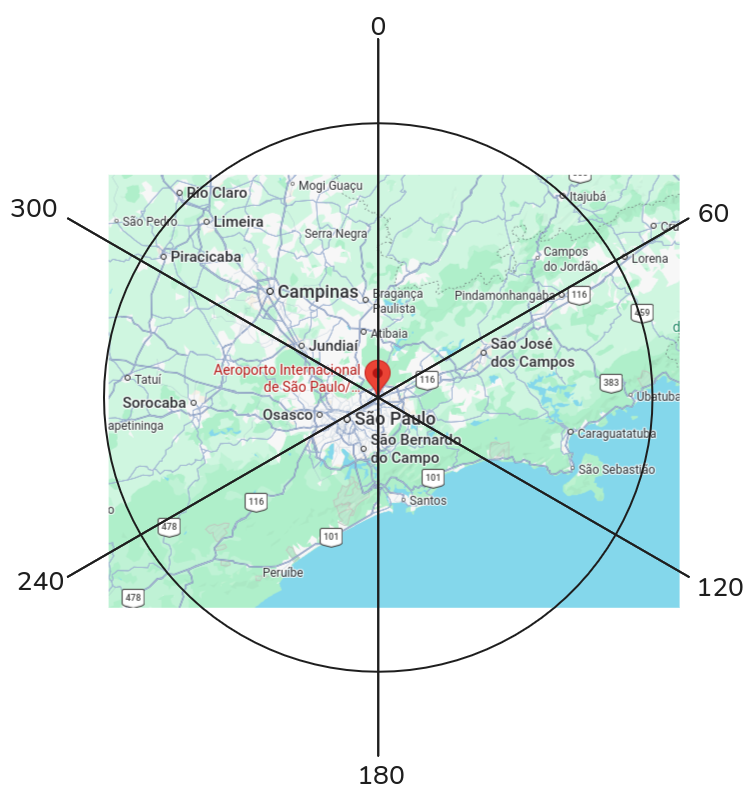
\includegraphics[width=0.8\linewidth]{images/gru_sectors.png}
    \caption{Guarulhos International Airport (GRU) Terminal Maneuvering Area (TMA) and its 60-degree entry sectors.}
    \label{fig:gru_sectors}
\end{figure}

Various factors can influence this indicator, including airspace design, meteorological conditions, and tactical interventions by Air Traffic Control (ATC) such as holding patterns and vectoring for sequencing. The comparison of the actual transit time to the 20th percentile baseline effectively isolates the operational inefficiencies, focusing on the ATM's responsibility in optimizing the arrival flow.

\subsubsection{KPI16: Additional Fuel Burn}
KPI16 represents the core metric for evaluating ATM-induced operational efficiency from an environmental perspective, providing an aggregate view of the excess fuel consumed during a flight phase. In the context of TMA operations, it is directly correlated with the inefficiencies captured by KPI08.

There are various methods for calculating KPI16. In Brazil, the Department of Air Space Control (DECEA) adopts a strategy similar to KPI08, as the additional fuel burn is calculated as the difference between the actual fuel consumed by an aircraft and a reference fuel consumption. Like KPI08, this baseline is determined as the 20th percentile of fuel consumption for similar flights. Positive values of KPI16 indicate fuel consumption above the expected optimal level—often resulting from airspace congestion and ATC interventions—whereas negative values indicate flights that operated more efficiently than the established baseline. As the target variable of the predictive models developed in this work, KPI16 serves as a direct proxy for the environmental and economic cost of ATM inefficiencies in the terminal area.

In this context, a shift can be observed from traditional approaches based on physico-mathematical models towards data-driven methodologies. Broadly, the literature can be organized into three main research streams: (i) aircraft performance modeling, (ii) operational analysis of Air Traffic Management (ATM), and (iii) the application of machine learning for fuel consumption and emissions estimation.

\subsection{Aircraft Performance Modeling}
The first research stream focuses on aircraft performance modeling. The Base of Aircraft Data (BADA) model, developed by EUROCONTROL \cite{nuic2010bada}, has become one of the primary references for aircraft performance studies, flight planning, trajectory simulation, and environmental assessments, providing widely used parametric performance models for ATM research. Subsequently, Del Pozo \textit{et al.} \cite{delpozo2022bada} proposed calibrating BADA coefficients using machine learning techniques and operational flight data, reducing discrepancies between nominal and observed in-service performance.

More recently, Jarry \textit{et al.} \cite{jarry2024generalization} investigated deep learning models for fuel flow estimation capable of generalizing across different aircraft types, while Jarry \textit{et al.} \cite{jarry2025ageing} incorporated engine ageing effects into fuel consumption modeling using Quick Access Recorder (QAR) data. In a similar vein, architectures based on Multi-Layer Perceptrons (MLP), Radial Basis Functions (RBF), and Recurrent Neural Networks (RNN) have been employed to develop tail-specific models \cite{hetherington2025tail}, exploiting QAR data to represent individual degradation and operational patterns.

Although these approaches achieve high accuracy in estimating fuel consumption, their application depends on high-frequency proprietary QAR data, which is typically unavailable to Air Navigation Service Providers (ANSPs). Furthermore, these models are primarily designed to represent the physical performance of individual aircraft rather than to estimate the operational fuel penalties arising from ATM inefficiencies. This limitation reduces their scalability and hinders their adoption in operational applications that rely exclusively on surveillance data and information routinely available to ANSPs.

\subsection{ATM Operational Analysis}
The second research stream investigates ATM operational efficiency. Kwasiborska and Skorupski \cite{kwasiborska2021merging} analyzed the environmental impact of different aircraft stream merging strategies during the approach phase, demonstrating that traffic flow organization directly influences additional flight time and, consequently, fuel consumption. In a complementary approach, Krauth \textit{et al.} \cite{krauth2023generative} developed a generative model based on Variational Autoencoders (VAEs) to generate realistic four-dimensional trajectories in Terminal Maneuvering Areas (TMAs), accounting for uncertainties arising from ATC interventions, meteorological conditions, and aircraft performance variability.

Although these studies contribute significantly to the understanding of air traffic dynamics and trajectory variability, their primary focus lies in trajectory simulation, operational flow analysis, and ATM scenario evaluation, rather than in the direct estimation of fuel penalties associated with ATM operational inefficiencies.

\subsection{Machine Learning for Fuel Consumption and Emissions Estimation}
A third research stream applies machine learning techniques to the estimation of fuel consumption and atmospheric emissions. Al Kazzaz \cite{alkazzaz2025emissions} developed an Artificial Neural Network (ANN) trained on data from the ICAO Engine Emissions Databank (EEDB) to predict fuel consumption and CO\textsubscript{2}, NO\textsubscript{x}, and CO emissions using engine parameters, fuel properties, and operational conditions. The study demonstrated that integrating ADS-B data, meteorological conditions, and engine characteristics can improve in-flight emission estimation. However, these studies concentrate on estimating aircraft atmospheric emissions rather than on quantifying the operational fuel penalties arising from ATM inefficiencies.

\subsection{Research Gap and Contribution}
Despite the advances observed across these research streams, an important gap remains in the literature. Existing studies focus predominantly on detailed aircraft performance modeling using proprietary on-board data such as QAR, on trajectory simulation, or on atmospheric emissions estimation. By contrast, few studies directly investigate the additional fuel consumption arising from ATM operational inefficiencies using exclusively operational data routinely available to ANSPs.

In this context, the present work proposes a machine learning–based approach to estimate Key Performance Indicator 16 (KPI16) using radar surveillance data, BADA performance parameters \cite{nuic2010bada}, ATM operational indicators, and meteorological information available prior to or at the moment of TMA entry. In contrast to Jarry \textit{et al.} \cite{jarry2024generalization, jarry2025ageing}, who focus on fuel flow modeling from high-fidelity QAR data; Krauth \textit{et al.} \cite{krauth2023generative}, whose focus lies in four-dimensional trajectory generation through generative models; and Al Kazzaz \cite{alkazzaz2025emissions}, whose work targets atmospheric emissions estimation, this study concentrates on predicting the additional fuel consumption associated with ATM operational inefficiencies. By integrating data sources routinely available to ANSPs, the proposed methodology advances the state of the art by enabling scalable KPI16 estimation applicable to the continuous monitoring of operational efficiency and environmental performance in terminal areas.

\section{PROPOSED APPROACH}
\label{sec:proposed_approach}

\subsection{Data Sources and Collection}
Data was collected from three main sources: surveillance radar data for civil flights landing in São Paulo/Guarulhos International Airport (ICAO: SBGR) was provided by Operational Data Integrator (ODIN) from Brazilian Airspace Control Institute (ICEA), flight-condition fuel usage for aircraft was extracted from Base of Aircraft Data (BADA) online API \cite{bada_a320} and climate data, including ceiling and visibility, was downloaded from Iowa State University API.

\subsubsection{ODIN Surveillance Radar Data}
ICEA's ODIN contains operational registries for air traffic all around Brazilian territory, including data from five radar arrays around Brazil: \textit{Amazônico} (located in north), \textit{Brasilia} (center-west), \textit{Recife} (northeast), \textit{Curitiba} (south) and \textit{Atlântico} (oceanic portion). They provide information for latitude, longitude, speed relative to sound, flight level, call sign registration and datetime for registry.

Also, ODIN provides previously calculated KPI08 data \cite{mca10022}, including departure airport, landing airport, call sign, weight class and type for aircraft, landing runway, datetime for entering in Terminal Maneuvering Area (TMA) and KPI08 metric itself \cite{doc9750}. Table \ref{tab:odin_dict} summarizes the specific fields from the ODIN surveillance and KPI08 datasets utilized in this work.

\begin{table}[htbp]
\caption{Data Dictionary for ODIN Surveillance Radar Data}
\label{tab:odin_dict}
\centering
\begin{tabular}{m{0.28\columnwidth} m{0.16\columnwidth} m{0.44\columnwidth}}
\hline
\textbf{Field} & \textbf{Type} & \textbf{Description} \\
\hline
\texttt{call\_sign} & String & Aircraft call sign registration \\
\texttt{adep} & String & Departure airport (ICAO code) \\
\texttt{ades} & String & Landing airport (ICAO code) \\
\texttt{aircraft\_type} & String & Aircraft model (e.g., A320) \\
\texttt{weight\_class} & String & Aircraft weight class (e.g., M, H) \\
\texttt{landing\_runway} & String & Validated landing runway (e.g., 09R) \\
\texttt{tma\_entry\_time} & Datetime & Datetime for entering the TMA \\
\texttt{kpi08} & Float & Calculated KPI08 metric (seconds) \\
\texttt{latitude} & Float & Aircraft latitude position \\
\texttt{longitude} & Float & Aircraft longitude position \\
\texttt{flight\_level} & Integer & Current flight level in hundreds of feet (e.g. 30) \\
\texttt{mach} & Float & Speed relative to sound (Mach) \\
\texttt{timestamp} & Datetime & Radar registry datetime \\
\hline
\end{tabular}
\end{table}

\subsubsection{BADA Efficiency Chart}
The aircraft efficiency map was computed using the Base of Aircraft Data (BADA) model \cite{bada_a320}, specifically BADA3, which accounts for, among other factors, the aircraft type and flight level in estimating instantaneous fuel consumption. The interface between the model and the study requirements was implemented through the \texttt{pyBADA} support library in Python \cite{pybada}. Table \ref{tab:bada_dict} presents the data dictionary for the BADA performance parameters extracted for our methodology.

\begin{table}[htbp]
\caption{Data Dictionary for BADA Efficiency Chart}
\label{tab:bada_dict}
\centering
\begin{tabular}{m{0.28\columnwidth} m{0.16\columnwidth} m{0.44\columnwidth}}
\hline
\textbf{Field} & \textbf{Type} & \textbf{Description} \\
\hline
\texttt{aircraft} & String & Aircraft model identifier (e.g., A320) \\
\texttt{tas\_ms} & Float & True Airspeed in meters per second \\
\texttt{fl} & Integer & Flight Level in hundreds of feet (e.g., 30) \\
\texttt{fuel\_flow\_kg\_s} & Float & Instantaneous fuel flow in kg/s \\
\hline
\end{tabular}
\end{table}

\subsubsection{Iowa State University Climate Data}
Iowa State University provides a public API for daily airport weather observations from around the world. In this article, studies will be focused on SBGR and will include both visibility and ceiling from observation radar. The specific fields retained from this dataset are described in Table \ref{tab:climate_dict}.

\begin{table}[htbp]
\caption{Data Dictionary for Iowa State University Climate Data}
\label{tab:climate_dict}
\centering
\begin{tabular}{m{0.28\columnwidth} m{0.16\columnwidth} m{0.44\columnwidth}}
\hline
\textbf{Field} & \textbf{Type} & \textbf{Description} \\
\hline
\texttt{valid} & Datetime & Observation timestamp (e.g., 2025-01-01 15:00) \\
\texttt{station} & String & Weather station ICAO code (e.g., SBSP) \\
\texttt{vsby} & Float & Visibility measurement (in miles) \\
\texttt{ceiling\_ft} & Float & Cloud ceiling height (in feet) \\
\hline
\end{tabular}
\end{table}

\subsection{Data Preparation and Feature Engineering}
The data for this paper were organized with possible scalability in mind. The source of the dataset is the Operational Data Integrator (ODIN) PostgreSQL database maintained by Brazilian Airspace Control Institute (ICEA); the records collected range from January 1 to December 31, 2025. Extraction was performed using Python scripts that produced Parquet files optimized for analytical workloads and stored locally. Subsequent data transformation employed DuckDB as the query engine, with transformations orchestrated through data build tool (dbt), forming a Medallion Architecture data pipeline \cite{databricks_medallion, saha_dataeng}. The resulting datasets were again exported as Parquet files for downstream analysis in Python. The stack used for this work is schematized on Figure \ref{fig:odin-etl-simplified}.

\begin{figure}[htbp]
    \centering
    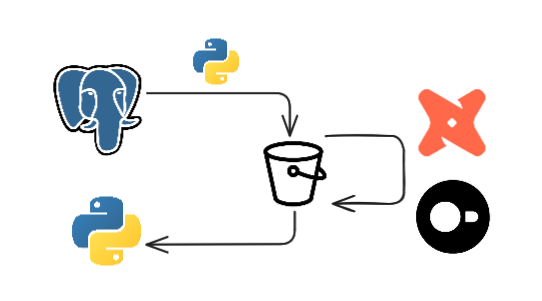
\includegraphics[width=1\linewidth]{images/odin-etl-simplified.png}
    \caption{Simplified schematics for the stack used in this work.}
    \label{fig:odin-etl-simplified}
\end{figure}

To enhance the analytical value of the flight data, a series of feature engineering transformations were applied using DuckDB and subsequently orchestrated and documented through dbt. We focused on creating features that better represented flight behavior, airspace congestion, and operational context.

The data transformations were structured across multiple SQL models to progressively build the final dataset:

\begin{itemize}
    \item \textbf{Trajectory Tracking and Elapsed Time:} The radar trajectory points were bounded between the time the aircraft crossed the TMA cylinder (\textit{c\_time}) and the actual landing time (\textit{aldt}). For each flight level (FL) recorded, the time difference between consecutive radar pings was calculated to establish the \textit{elapsed} time spent at each altitude.
    
    \item \textbf{Fuel Consumption Estimation:} The \textit{elapsed} time per flight level was multiplied by the aircraft's specific average fuel flow rate (kg/s) obtained from the BADA performance tables \cite{bada_a320, pybada}. The sum of these values across all flight levels yielded the total fuel consumption in the terminal area (\textit{consumption\_kg}).
    
    \item \textbf{Airspace Congestion Tracking:} To represent the dynamic traffic density, an event-based running sum was implemented. Every \textit{c\_time} was treated as an entry (+1) and every \textit{aldt} as an exit (-1). Using SQL window functions over the chronological timeline, we calculated the exact number of aircraft present in the TMA at any given moment (\textit{nr\_aircraft\_in\_tma}).
    
    \item \textbf{Rolling Predictive Metrics:} A moving average for the time spent in the TMA (\textit{transit\_tma\_predicted}) was created to mimic the expected transit time given recent conditions. This was calculated over a 1-hour rolling window preceding the flight, partitioned by the validated runway (\textit{drwy\_validado}) and the entry sector (\textit{setor}).
    
    \item \textbf{Baseline Efficiency and Target Variable:} To define a standard for efficient operations, we calculated the 20th percentile of fuel consumption (\textit{consumption\_20p}) partitioned by departure airport (\textit{adep}), aircraft type, and landing runway. Finally, the main target variable for this study, \textit{kpi16}, was computed as the difference between the actual fuel consumption (\textit{consumption\_kg}) and this 20th percentile baseline.
    
    \item \textbf{Temporal and Environmental Variables:} Datetime fields were decomposed into specific categories (\textit{day}, \textit{month}, \textit{hour}, and \textit{day of week}) to capture seasonal and daily patterns. Additionally, weather information from the METAR database (Iowa State University public API) was joined by the hour, incorporating horizontal visibility and cloud ceiling to assess their impact on flight holding and routing.
\end{itemize}

These transformations—ranging from chronological event tracking to percentile-based baselining—were carefully designed to expose underlying trends, airspace bottlenecks, and correlations within the flight data, paving the way for sophisticated machine learning investigations. Furthermore, adopting structured data modeling approaches (e.g., Medallion architecture) ensures scalability when applying these pipelines to massive Apache Spark or distributed SQL environments \cite{databricks_medallion, saha_dataeng}.

After the data transformation process, the variables can be classified into five main categories based on their purpose:
\begin{itemize}
    \item \textbf{Identification and temporal:} Unique flight identifier ($id$), date ($date$), day of the month ($day$), month ($month$), hour ($hour$), and day of the week ($dow$).
    \item \textbf{Operational:} Departure airport ($adep$), aircraft type ($aircraft$), validated landing runway ($drwy\_validado$), and TMA entry sector ($setor$).
    \item \textbf{Traffic and flight time:} Total transit time in TMA ($transit\_tma$), additional transit time ($kpi08$), number of aircraft in TMA ($nr\_aircraft\_in\_tma$), and predicted average transit time ($transit\_tma\_predicted$).
    \item \textbf{Meteorological:} Horizontal visibility ($visibility$) and cloud ceiling ($ceiling$).
    \item \textbf{Fuel consumption:} Total consumption in TMA ($consumption\_kg$), 20th percentile reference consumption ($consumption\_20p$), and additional consumption ($kpi16$).
\end{itemize}

\subsection{Exploratory Data Analysis}
The final dataset comprises 64,119 flight records representing landing operations at Guarulhos International Airport (SBGR) collected between January and December 2025. The dataset includes temporal, operational, traffic, meteorological, and fuel-consumption-related variables. An exploratory data analysis (EDA) was conducted to investigate the distribution of KPI16 and its relationship with the explanatory variables, as well as identify relevant patterns and highlight relationships that might influence the additional fuel consumption (KPI16) in the terminal area.

The distribution of $kpi16$ presents elongated tails, as shown in Figure \ref{fig:kpi16-distribution}, indicating the presence of observations with significantly high additional consumption. Such cases may be associated with adverse operational conditions, such as airspace congestion, unfavorable weather, or prolonged holding procedures. Outlier analysis was handled conservatively, maintaining observations between the 1st and 99th percentiles to preserve extreme events that represent actual operational behavior within the system.

\begin{figure}[htbp]
    \centering
    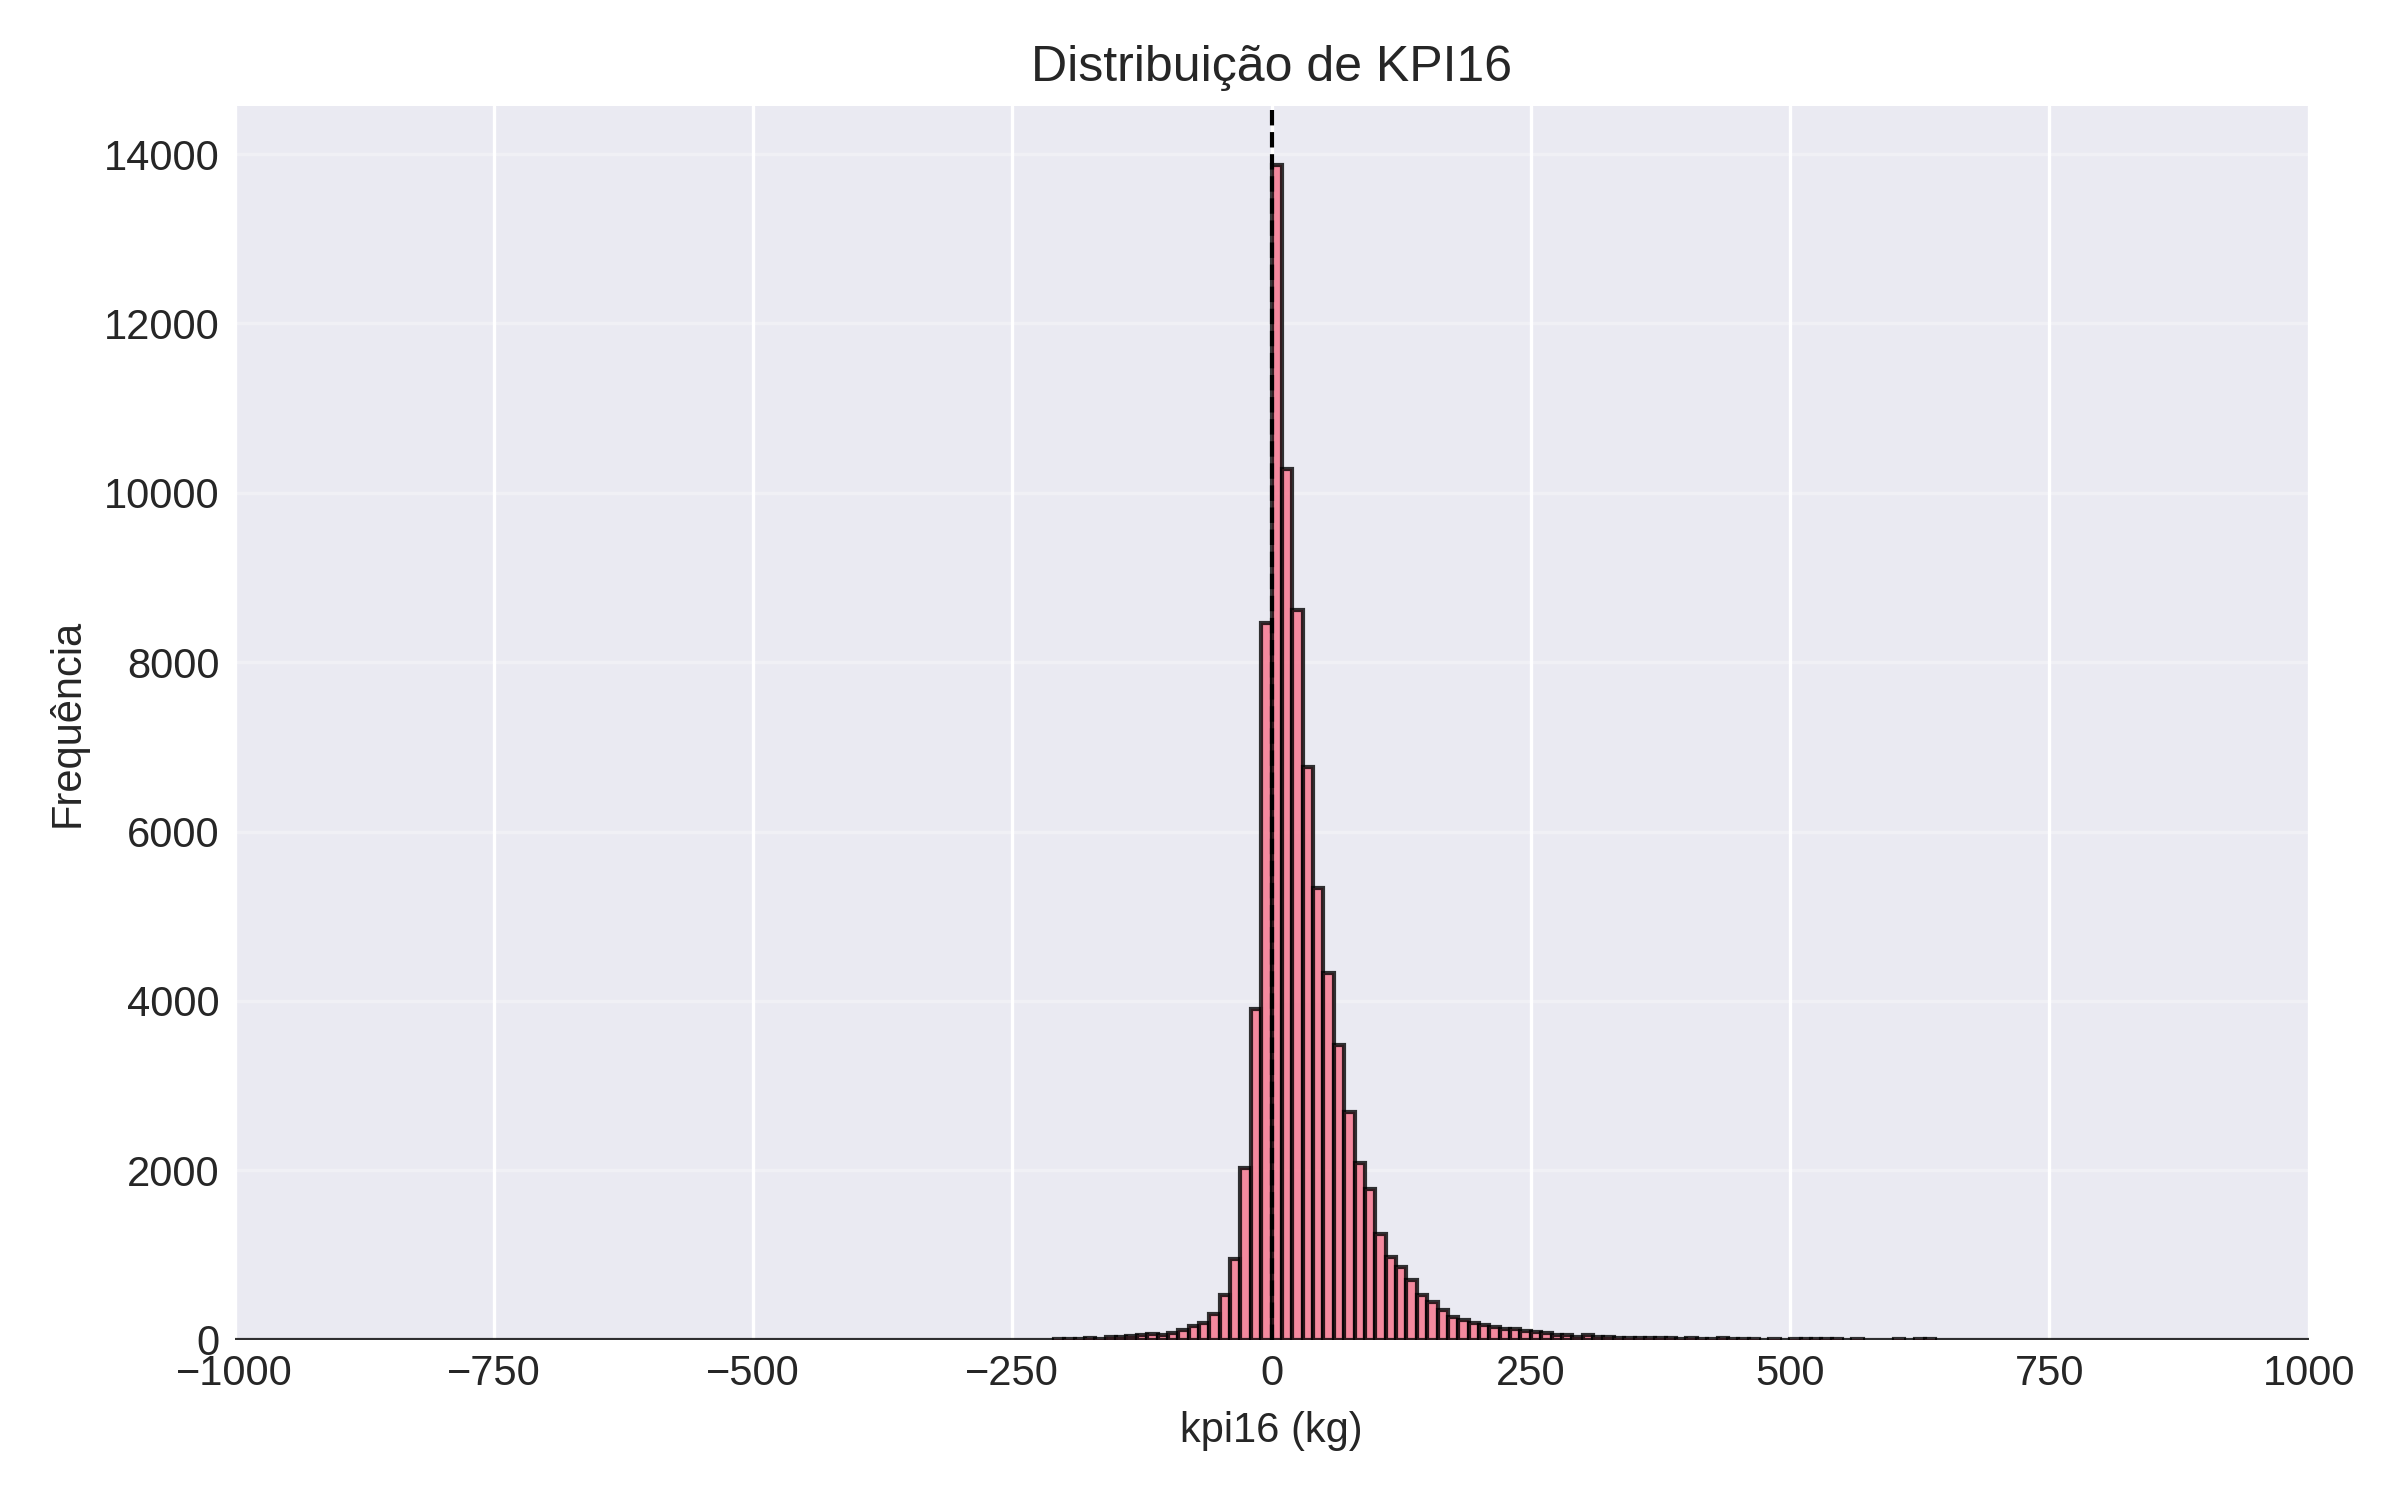
\includegraphics[width=1\linewidth]{images/kpi16-distribution.png}
    \caption{Distribution of the target variable $kpi16$ (Additional Fuel Consumption).}
    \label{fig:kpi16-distribution}
\end{figure}

\subsubsection{Additional Fuel Consumption by Departure Airport}
The departure airport (ADEP) plays a critical role in shaping the flight profile, cruise altitude, and approach procedure into the destination TMA. Figure \ref{fig:adep-kpi16} highlights the average additional fuel consumption (KPI16) for the 15 most frequent ADEPs. Notably, flights originating from Afonso Pena International Airport (SBCT) in Curitiba and Hercílio Luz International Airport (SBFL) in Florianópolis present the highest average penalties. This pattern suggests that these airports may share approach-related challenges, possibly associated with their geographical proximity and common entry routing into the Guarulhos TMA.

\begin{figure}[htbp]
    \centering
    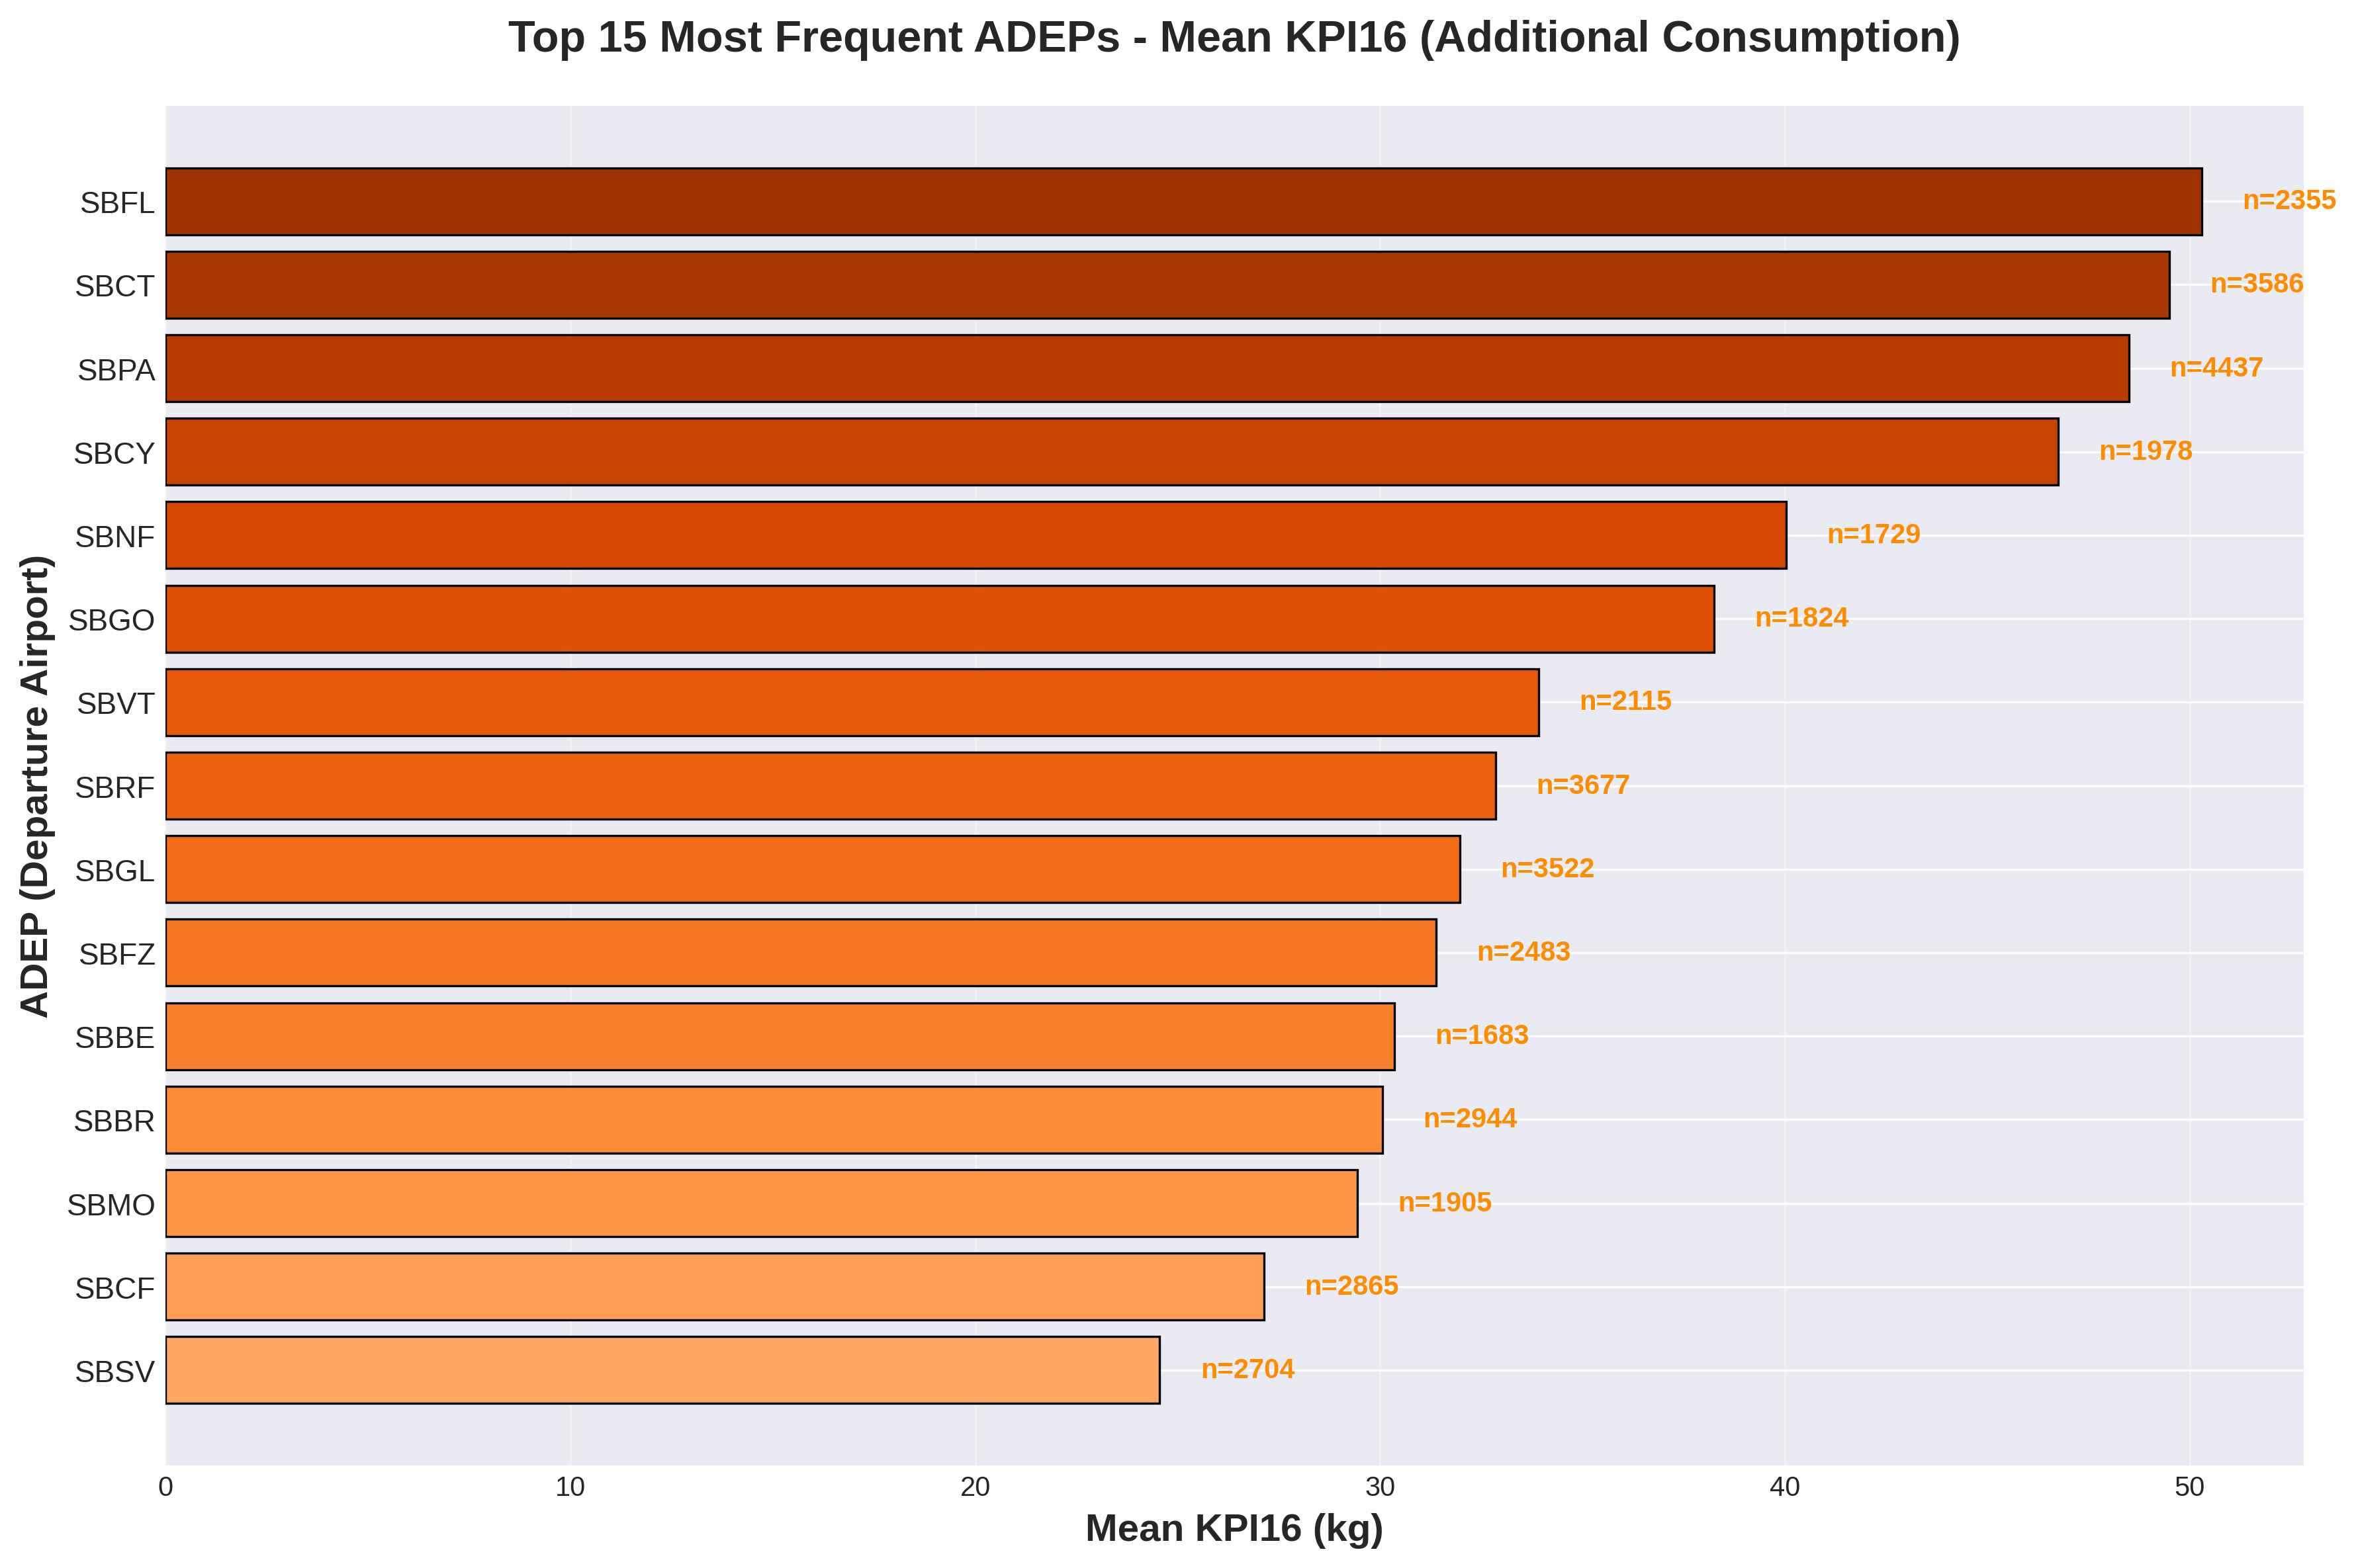
\includegraphics[width=1\linewidth]{images/adep_kpi16.png}
    \caption{Average additional fuel consumption (KPI16) by Departure Airport (ADEP).}
    \label{fig:adep-kpi16}
\end{figure}

\subsubsection{Impact of TMA Entry Sector on Efficiency}
To further investigate the geographical bottlenecks, the TMA was divided into entry sectors of 60-degree increments based on the aircraft's bearing upon crossing the terminal cylinder (excluding sector 120.0 due to insufficient sample size). As demonstrated in Figure \ref{fig:setor-kpi16}, flights entering through Sector 180.0 and Sector 300.0 demand the highest additional fuel consumption.

This pattern suggests that flights entering through these sectors may be associated with operational conditions that result in higher additional fuel consumption.

\begin{figure}[htbp]
    \centering
    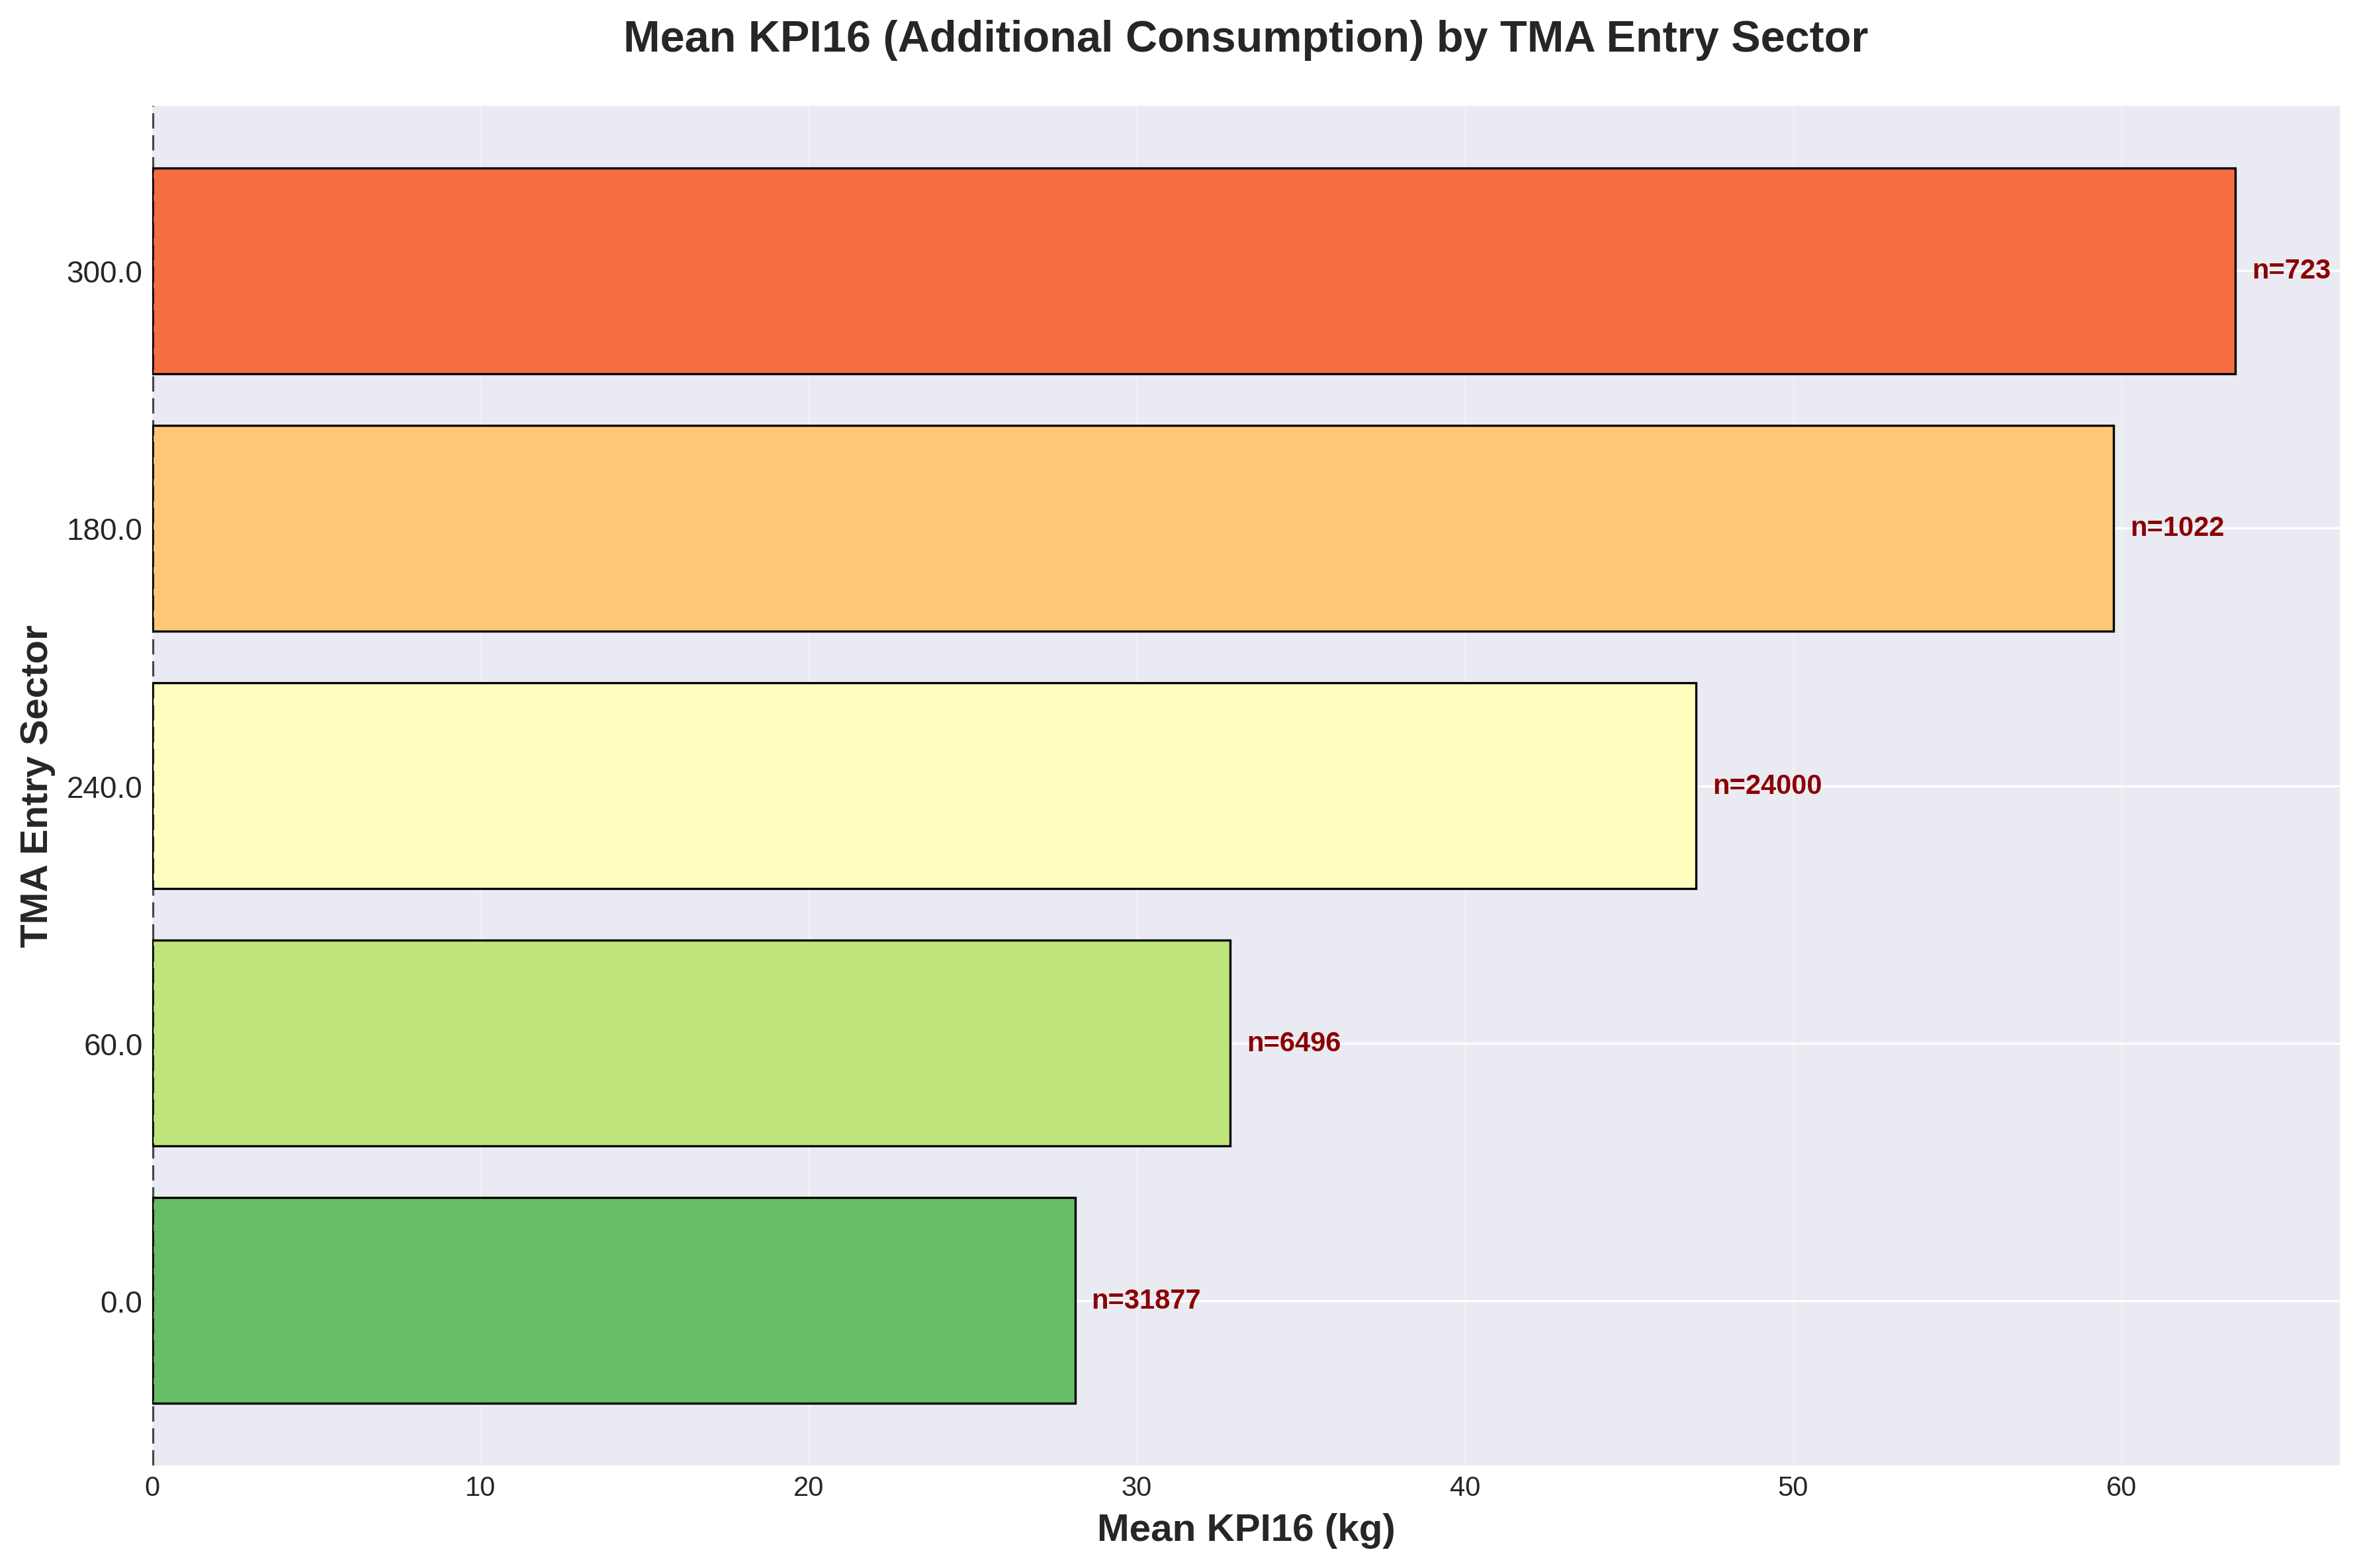
\includegraphics[width=1\linewidth]{images/setor_kpi16.png}
    \caption{Mean KPI16 (Additional Consumption) distributed by TMA Entry Sector.}
    \label{fig:setor-kpi16}
\end{figure}

\subsubsection{Interaction Between Entry Sectors and Origin Airports}
A more granular analysis combining both origin airports and entry sectors offers additional insight into factors that may contribute to the aforementioned inefficiencies. Figure \ref{fig:setor-adep-kpi16} details the most frequent ADEPs for the most penalizing sectors. Sector 180.0 is predominantly associated with flights from Southern capitals (Florianópolis, Porto Alegre, and Curitiba), while Sector 300.0 handles traffic from Goiânia, Uberlândia, and Manaus. The elevated additional fuel consumption observed in these sectors suggests that flights originating from these locations may be subject to more complex operational conditions within the TMA. One possible explanation is the convergence of multiple traffic flows into the same entry sectors, potentially increasing the complexity of arrival management and contributing to greater operational delays.

\begin{figure}[htbp]
    \centering
    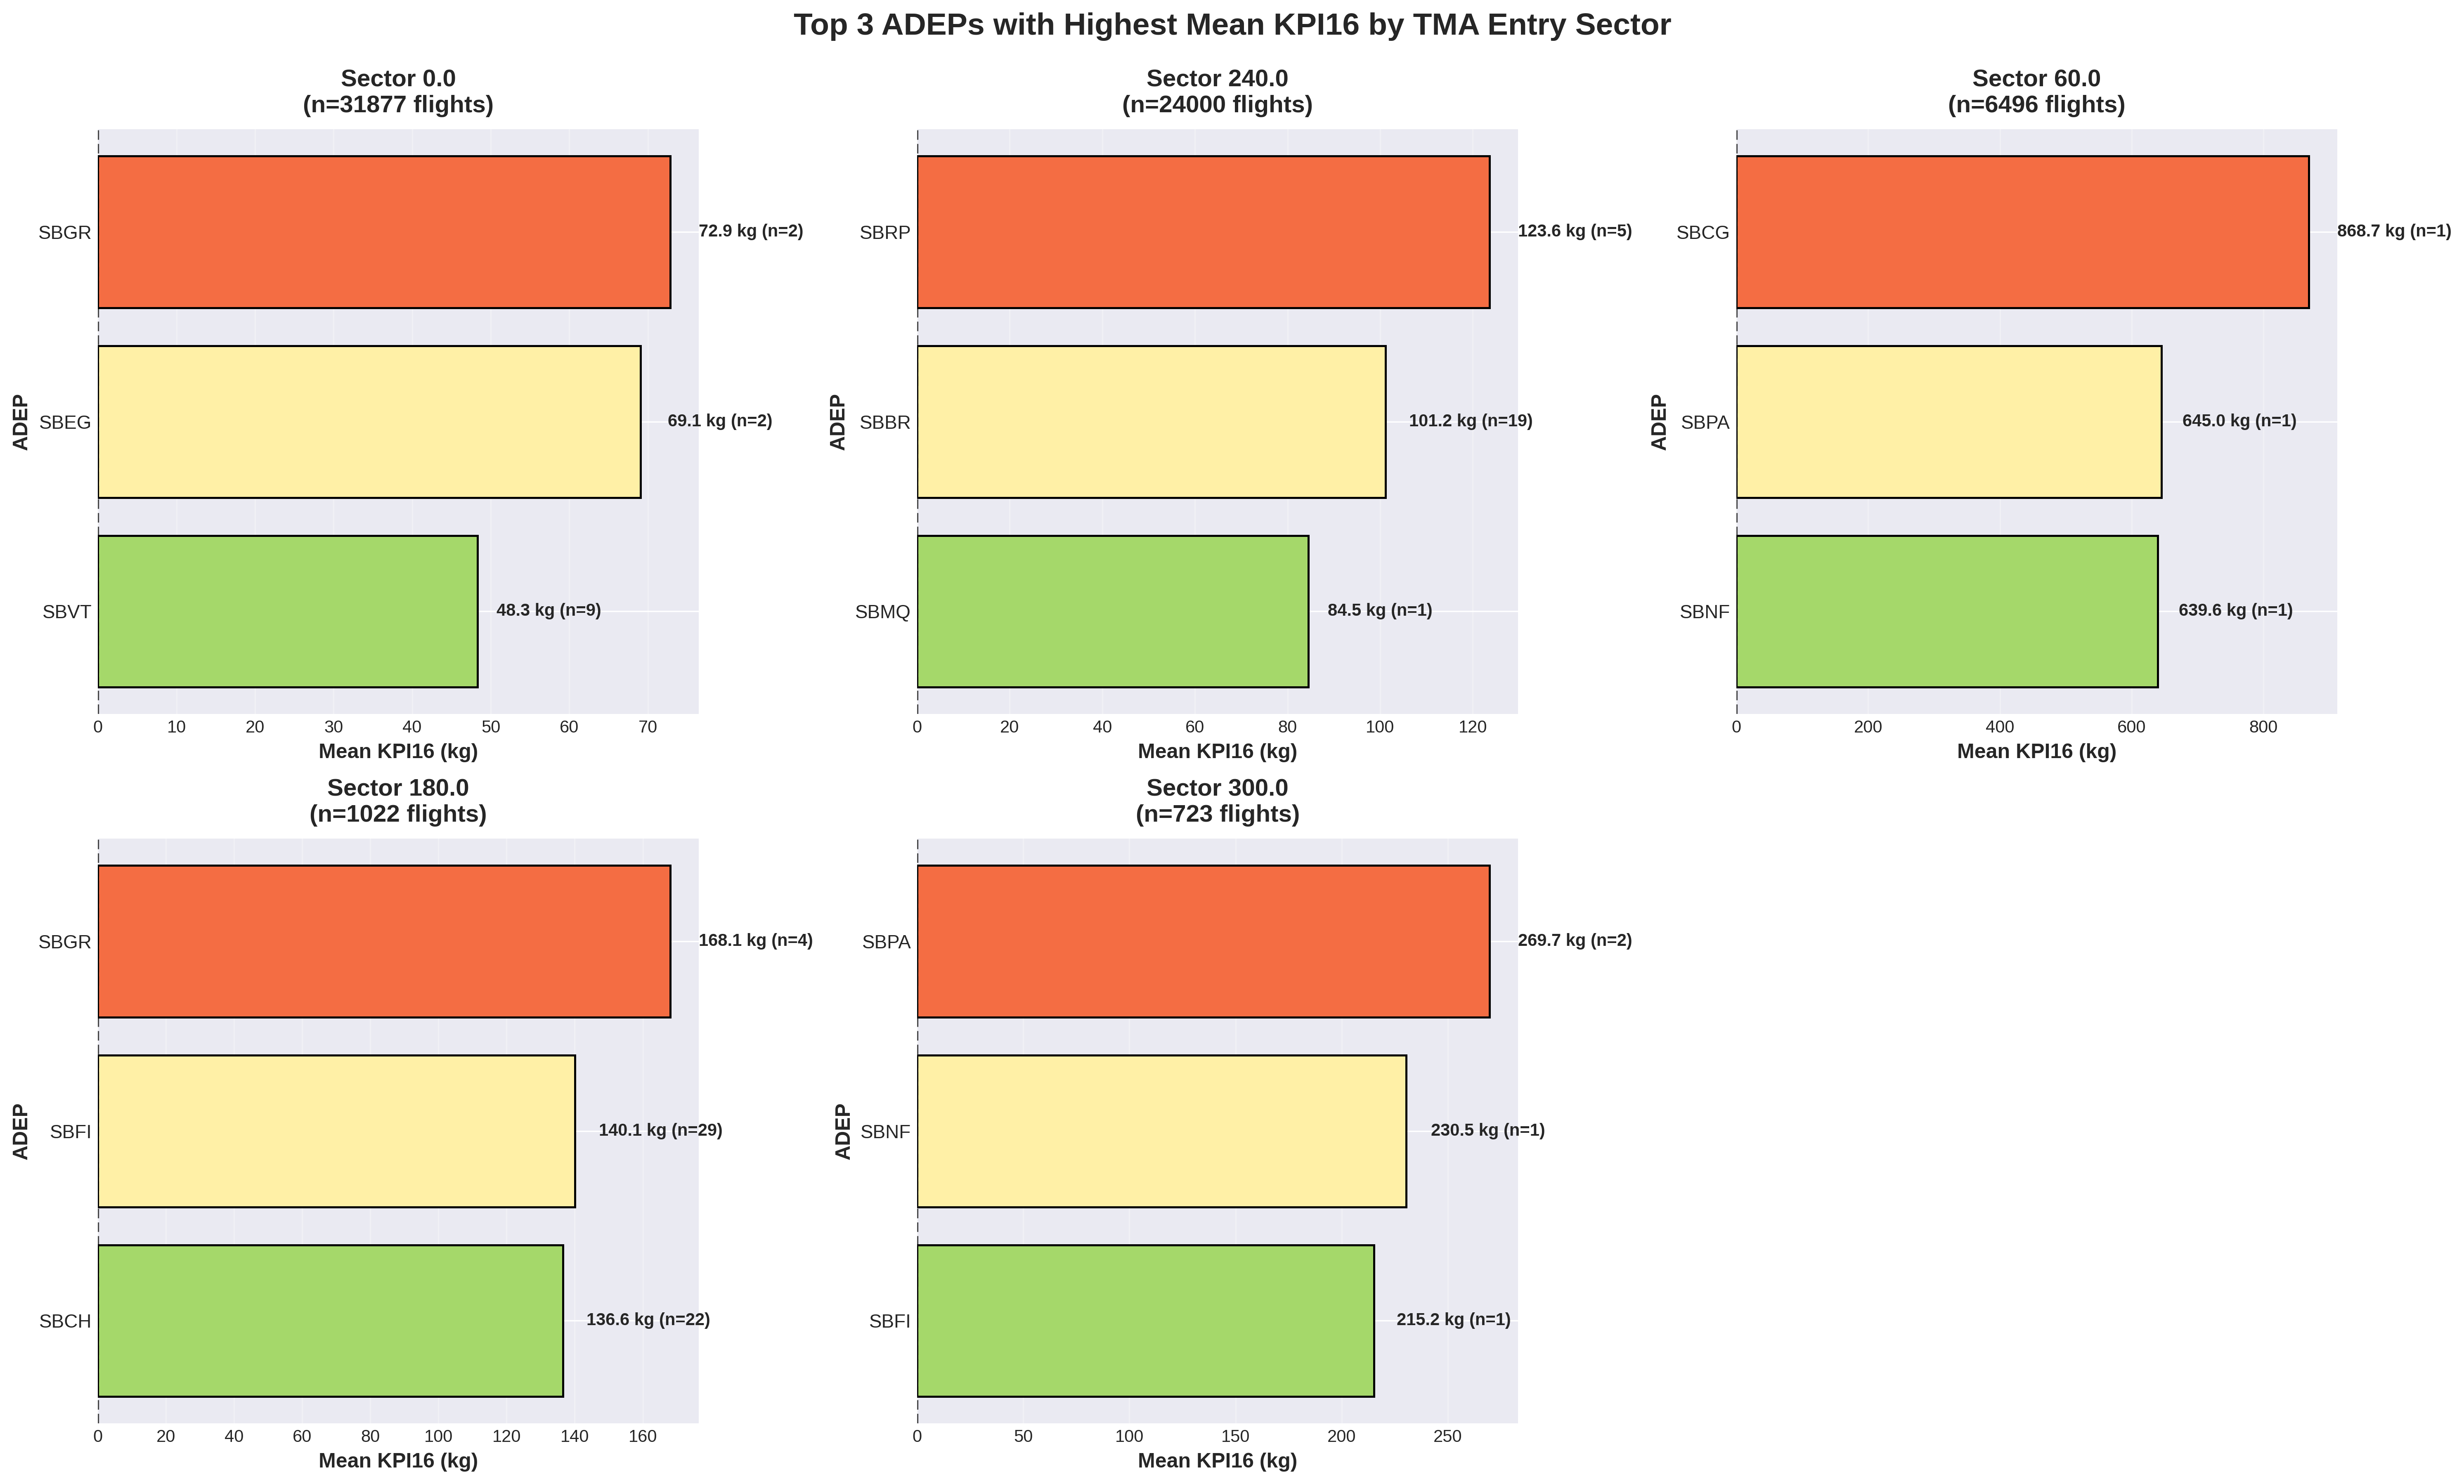
\includegraphics[width=1\linewidth]{images/setor_adep_kpi16.png}
    \caption{Top ADEPs contributing to high KPI16, grouped by TMA Entry Sector.}
    \label{fig:setor-adep-kpi16}
\end{figure}

To further support this observation, Figure \ref{fig:common-adep-sector} presents the share of total entries into each TMA entry sector attributed to the most frequent ADEPs. Notably, SBPA, SBCT, and SBFL together account for a dominant proportion of traffic entering through Sector 180, constituting evidence of traffic concentration rather than a confirmed causal mechanism. This concentration pattern may contribute to increased arrival management complexity, particularly when these flows overlap during peak periods.

\begin{figure}[htbp]
    \centering
    \includesvg[width=1\linewidth]{images/common_adep_sector}
    \caption{Share of total entries into each TMA entry sector by most frequent ADEPs, highlighting the dominant contribution of SBPA, SBCT, and SBFL to Sector 180 traffic volume.}
    \label{fig:common-adep-sector}
\end{figure}

\subsubsection{Hourly Traffic Variations and Congestion Cascading}
Air traffic operates in waves, and the time of arrival heavily dictates the level of congestion encountered. Figure \ref{fig:hora-adep} groups the performance of the three most impactful ADEPs across the six busiest hours of the day. During peak periods, flights originating from SBPA, SBCT, and SBFL appear to concentrate in Sector 180, which may increase the operational complexity of the traffic and contribute to the higher KPI16 values observed in the flow. Consequently, flights from Florianópolis (SBFL) sharing the same entry sector are often associated with elevated fuel penalties, suggesting a cascading effect on overall performance.

\begin{figure}[htbp]
    \centering
    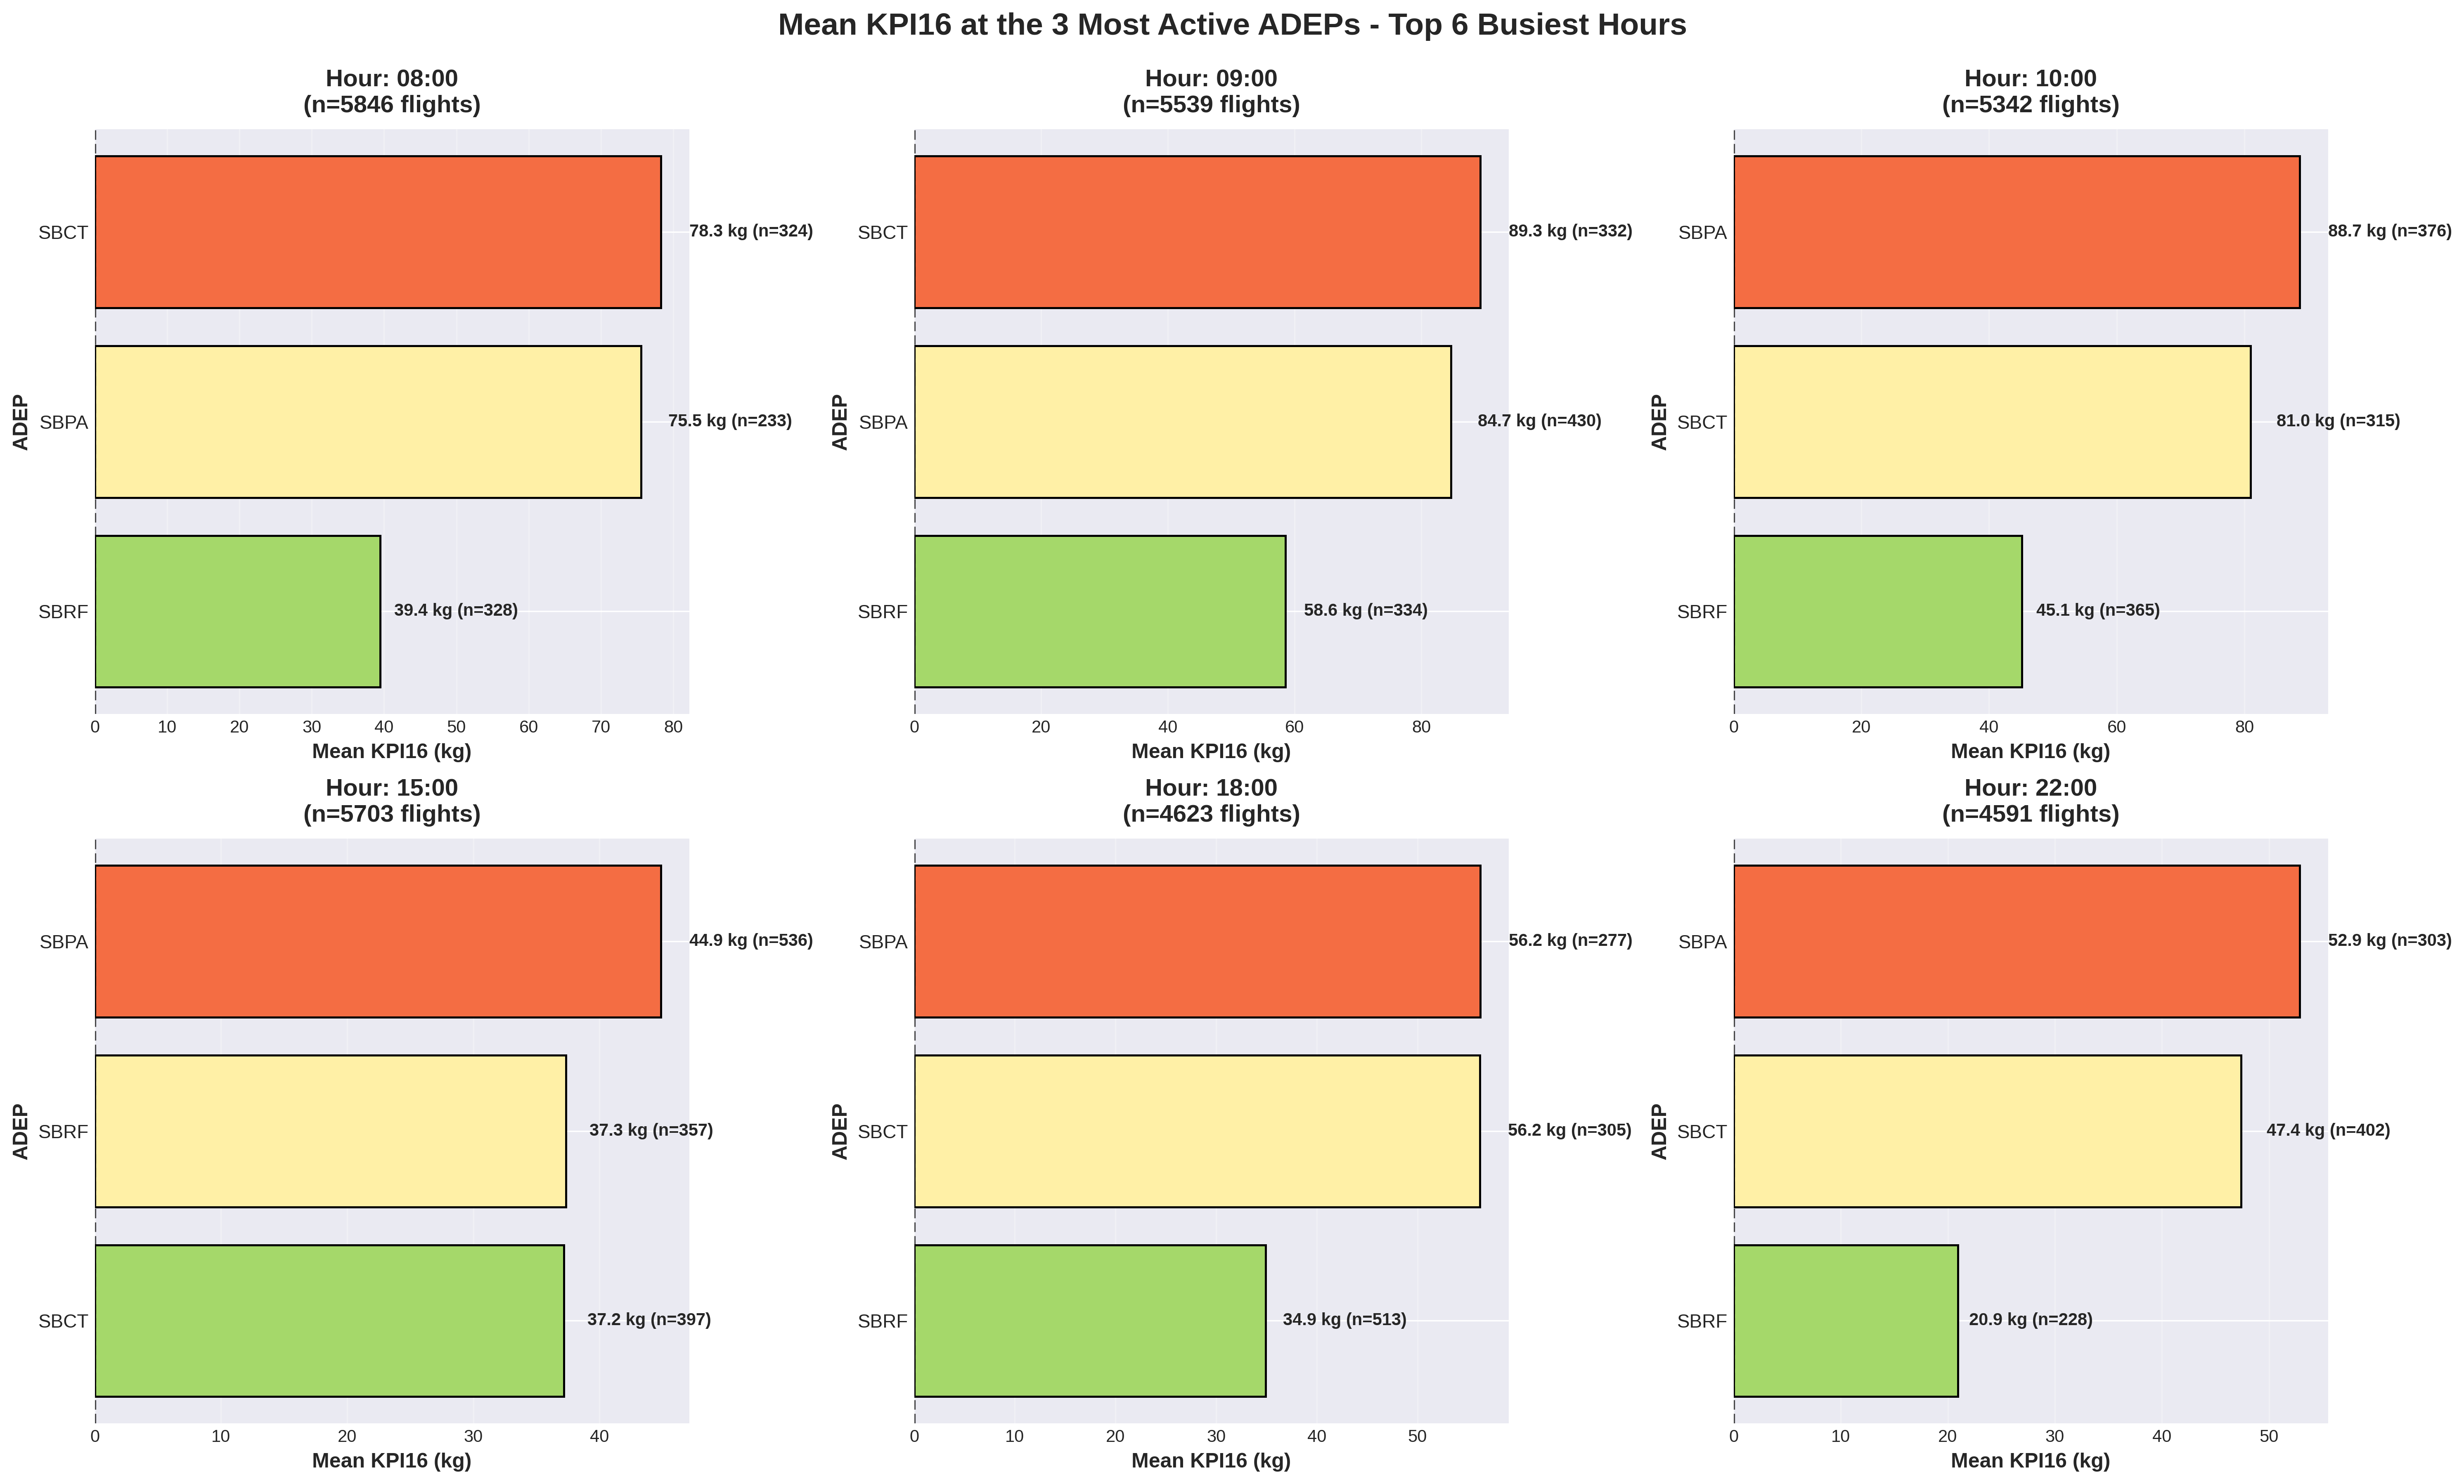
\includegraphics[width=1\linewidth]{images/hora_adep.png}
    \caption{Mean KPI16 for the three most active ADEPs during the top six busiest landing hours.}
    \label{fig:hora-adep}
\end{figure}

\subsection{Machine Learning Approach}
To evaluate the predictability of the additional fuel consumption ($kpi16$) given the operational, spatial, and meteorological conditions prior to or at the exact moment the aircraft enters the Terminal Control Area (TMA), we formulated the problem as a supervised machine learning regression task.

A rigorous pipeline was established to prevent data leakage: features that could only be observed after the flight's landing (e.g., total transit time, actual fuel consumed) were strictly excluded from the predictive models. This ensures the integrity of time-series estimations, a common pitfall observed in environmental and operational monitoring tasks \cite{dataleakage}. The final set of explanatory variables included both numerical features (e.g., number of concurrent aircraft in the TMA, predicted transit time based on a rolling window, visibility, and cloud ceiling) and categorical features (e.g., origin airport, aircraft type, entry sector, validated runway, month, hour, and day of the week).

Missing values in the cloud ceiling variable were imputed with a constant high value (10,000 ft) assuming clear sky conditions, while other numerical variables were imputed using their respective medians. For the baseline linear model, categorical features were encoded using One-Hot Encoding and numerical features were normalized using Standard Scaling. For a fair and direct comparison, this exact same pre-processed dataset was utilized across all evaluated algorithms, employing a randomized train-test split with an 80/20 ratio (51,295 records for training and 12,824 for testing).

We benchmarked six distinct machine learning algorithms to map the complex, non-linear relationships of airspace congestion to fuel consumption.

\subsubsection{Linear Regression (Baseline)}
To establish a performance baseline, an Ordinary Least Squares (OLS) Linear Regression \cite{hastie2009elements} was trained. While highly interpretable and computationally efficient, linear regression assumes a linear relationship between the predictors and the target variable. In highly complex environments like air traffic management, this model serves as a simple and interpretable benchmark.

\subsubsection{Random Forest Regressor}
Random Forest \cite{breiman2001random} is a robust ensemble learning method that operates by constructing a multitude of decision trees during training and outputting the average prediction of the individual trees. It uses a bagging (bootstrap aggregating) technique to reduce variance and avoid overfitting. We configured the model with 100 estimators and a maximum depth of 15 to balance model complexity and generalization capacity.

\subsubsection{Gradient Boosting Regressor}
Gradient Boosting \cite{friedman2001greedy} is a sequential ensemble technique where each new decision tree is trained to correct the residual errors made by the previous trees. It is highly effective for tabular data with heterogeneous features. The Scikit-Learn implementation of the Gradient Boosting Regressor was trained using 100 estimators, a learning rate of 0.1, and a maximum tree depth of 5.

\subsubsection{XGBoost}
Extreme Gradient Boosting (XGBoost) \cite{chen2016xgboost} was selected due to its proven performance on structured tabular datasets and its ability to model complex nonlinear interactions between traffic, operational, and meteorological variables. It incorporates advanced regularization (L1 and L2) to prevent overfitting. For our tabular dataset, we utilized the histogram-based tree method (\texttt{tree\_method='hist'}), which significantly speeds up the training process. The model was parametrized identically to the standard Gradient Boosting (100 estimators, learning rate of 0.1, maximum depth of 5).

\subsubsection{LightGBM}
Light Gradient Boosting Machine (LightGBM) \cite{ke2017lightgbm}, developed by Microsoft, is a gradient boosting framework that uses tree-based learning algorithms. It is designed for distributed and efficient training, notably using a leaf-wise (rather than level-wise) tree growth strategy. This allows for faster convergence and lower memory usage. We trained the LightGBM model with 100 estimators, a learning rate of 0.1, and a maximum depth of 5.

\subsubsection{CatBoost}
Categorical Boosting (CatBoost) \cite{prokhorenkova2018catboost}, developed by Yandex, is an algorithm that natively handles categorical variables without the need for extensive pre-processing (like One-Hot Encoding). It uses oblivious decision trees, which decreases scoring time and avoids overfitting. Although CatBoost is capable of processing raw categorical data, we trained it on our pre-processed dataset for a strict one-to-one benchmark. The model was configured with 100 iterations, a learning rate of 0.1, and a depth of 5.

\section{EXPERIMENTS AND RESULTS}
\label{sec:experiments_results}

\subsection{Experimental Results}
The performance of the predictive models was evaluated using the Root Mean Squared Error (RMSE), the Mean Absolute Error (MAE), and the Coefficient of Determination ($R^2$). The $R^2$ score represents the proportion of the variance in the dependent variable that is predictable from the independent variables, whereas RMSE and MAE measure the average magnitude of the errors in kilograms of fuel.

The consolidated results of the models evaluated on the test set are presented in Table \ref{tab:models_summary}.

\begin{table}[htbp]
\caption{Comparison of Machine Learning Models}
\label{tab:models_summary}
\centering
\begin{tabular}{lccc}
\hline
\textbf{Model} & \textbf{RMSE} & \textbf{MAE} & \textbf{$R^2$} \\
\hline
Gradient Boosting & 35.19 & 22.71 & 0.5887 \\
XGBoost & 35.31 & 22.70 & 0.5858 \\
LightGBM & 35.34 & 22.72 & 0.5852 \\
Random Forest & 35.44 & 22.87 & 0.5829 \\
CatBoost & 36.07 & 23.28 & 0.5679 \\
Linear Regression & 38.23 & 24.60 & 0.5147 \\
\hline
\end{tabular}
\end{table}

\begin{figure}[htbp]
    \centering
    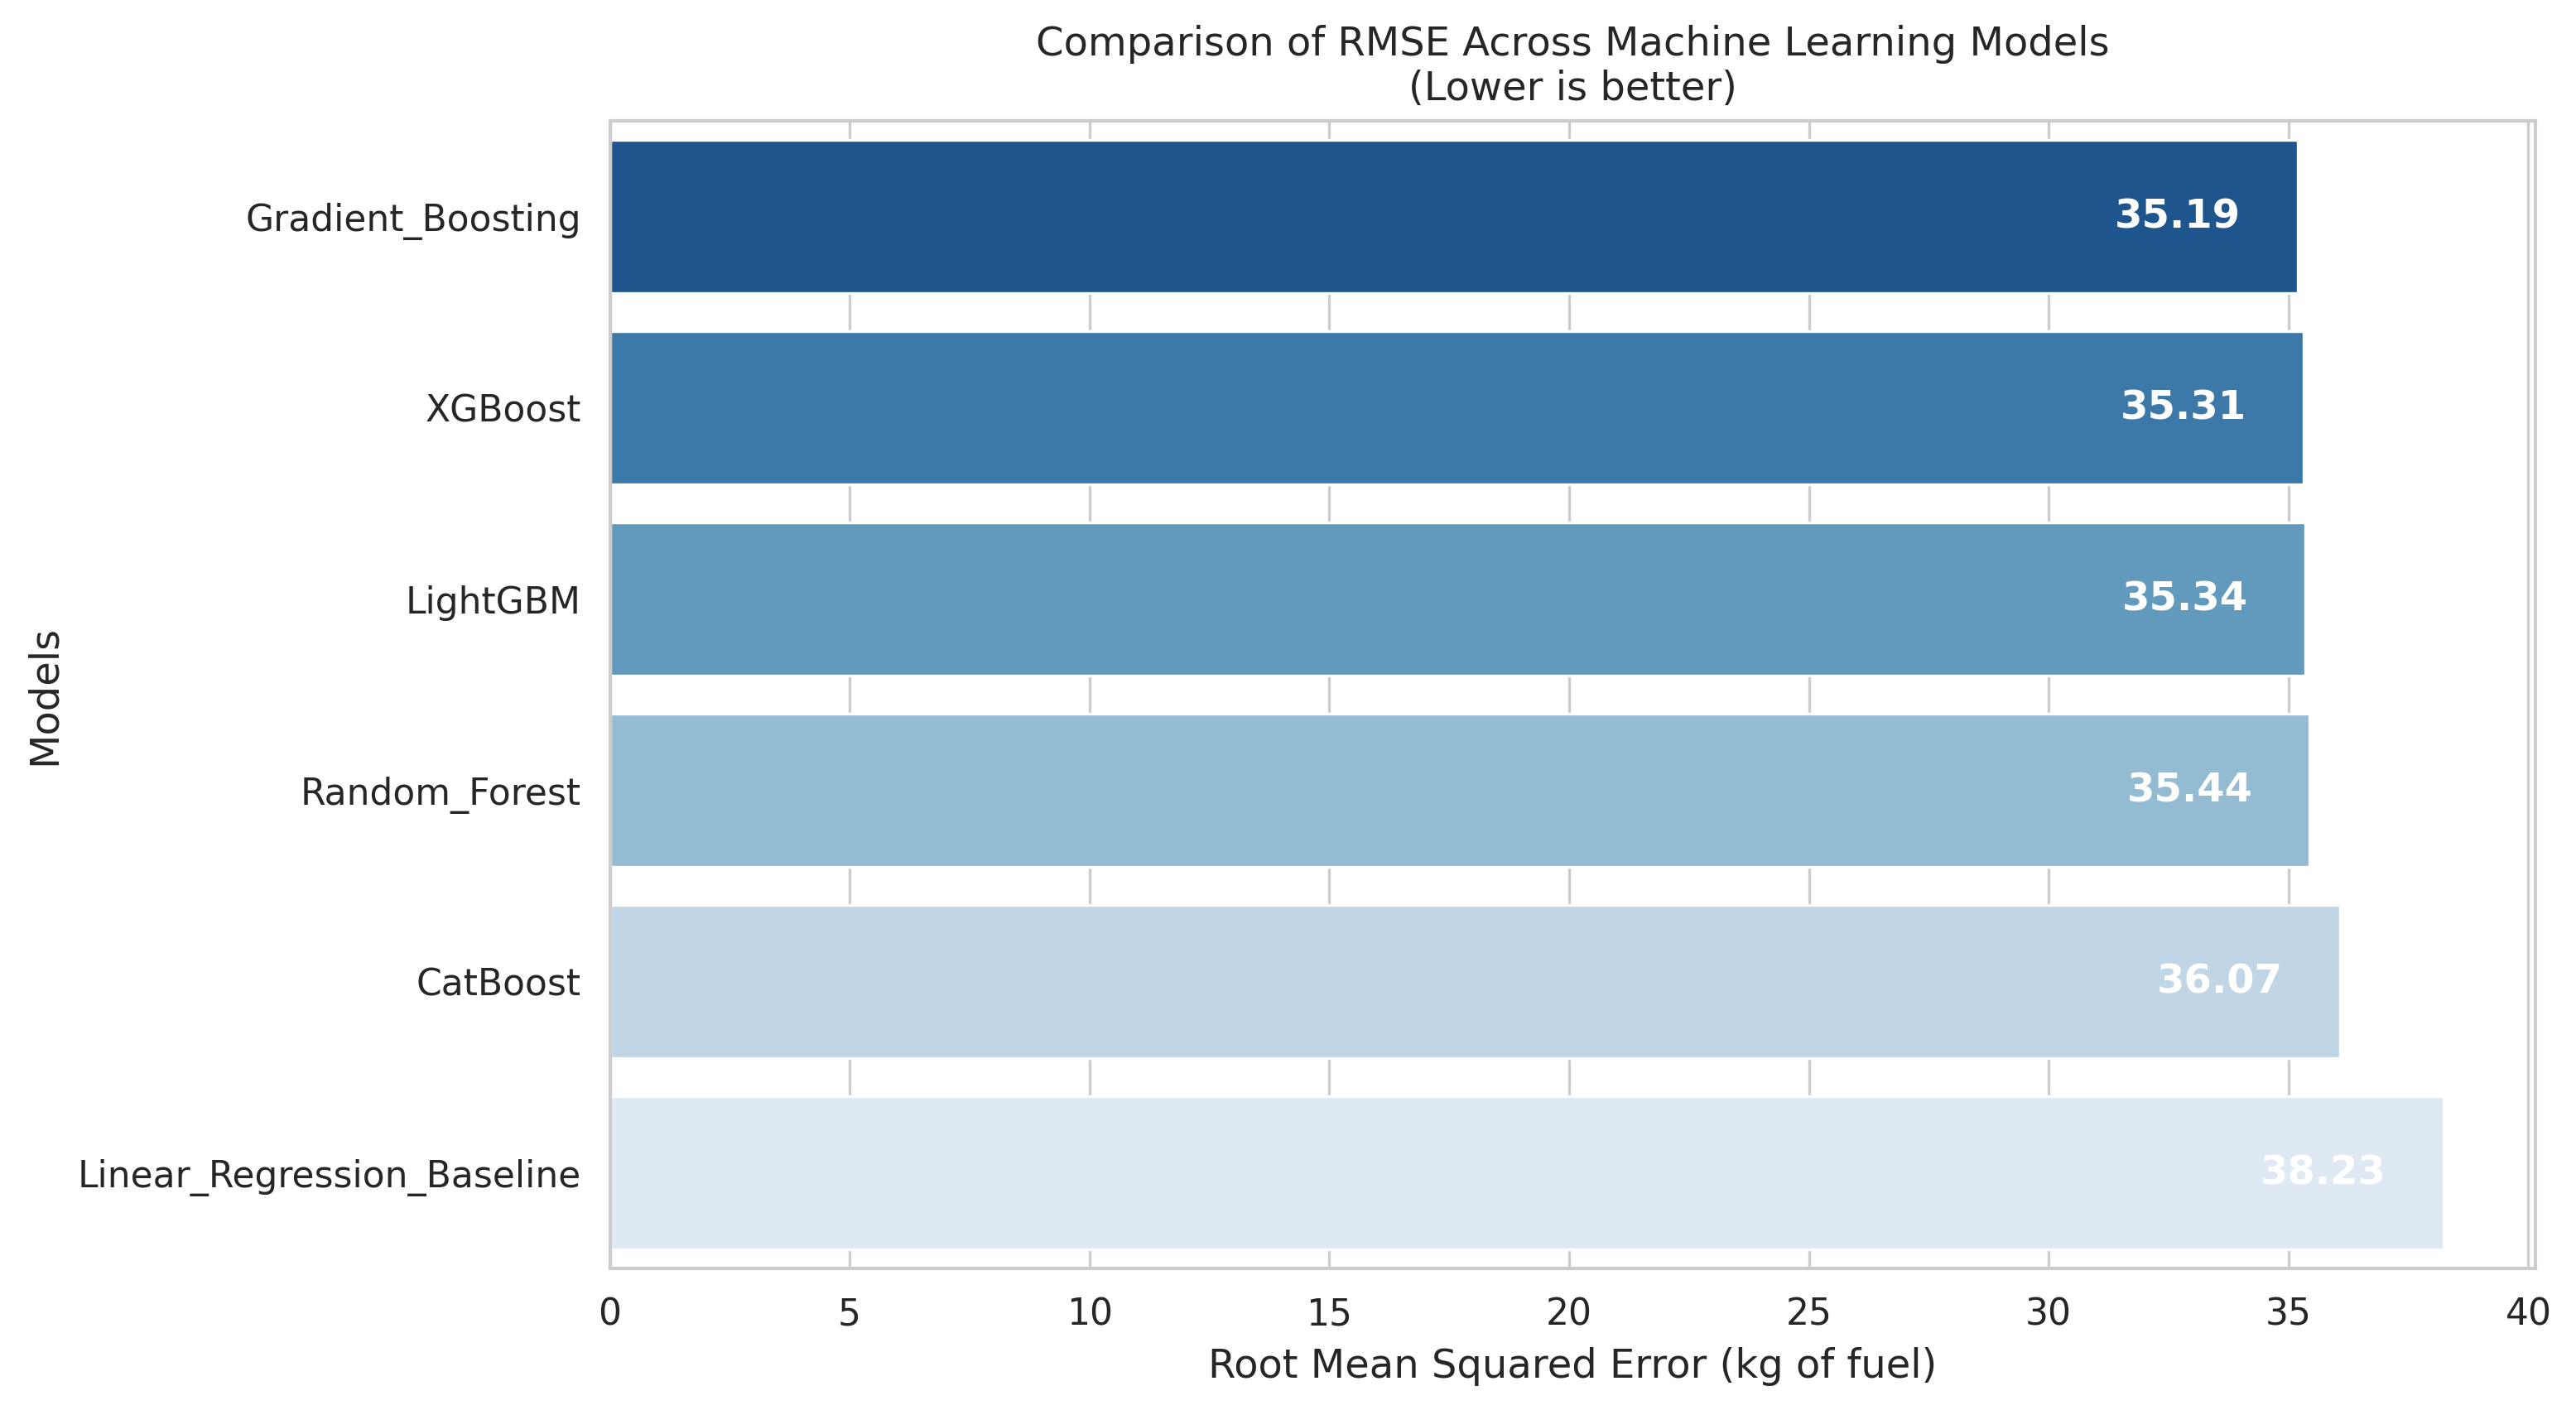
\includegraphics[width=1\linewidth]{images/comparativo_rmse.png}
    \caption{Root Mean Squared Error (RMSE) comparison across the evaluated machine learning models.}
    \label{fig:comparativo_rmse}
\end{figure}

\begin{figure}[htbp]
    \centering
    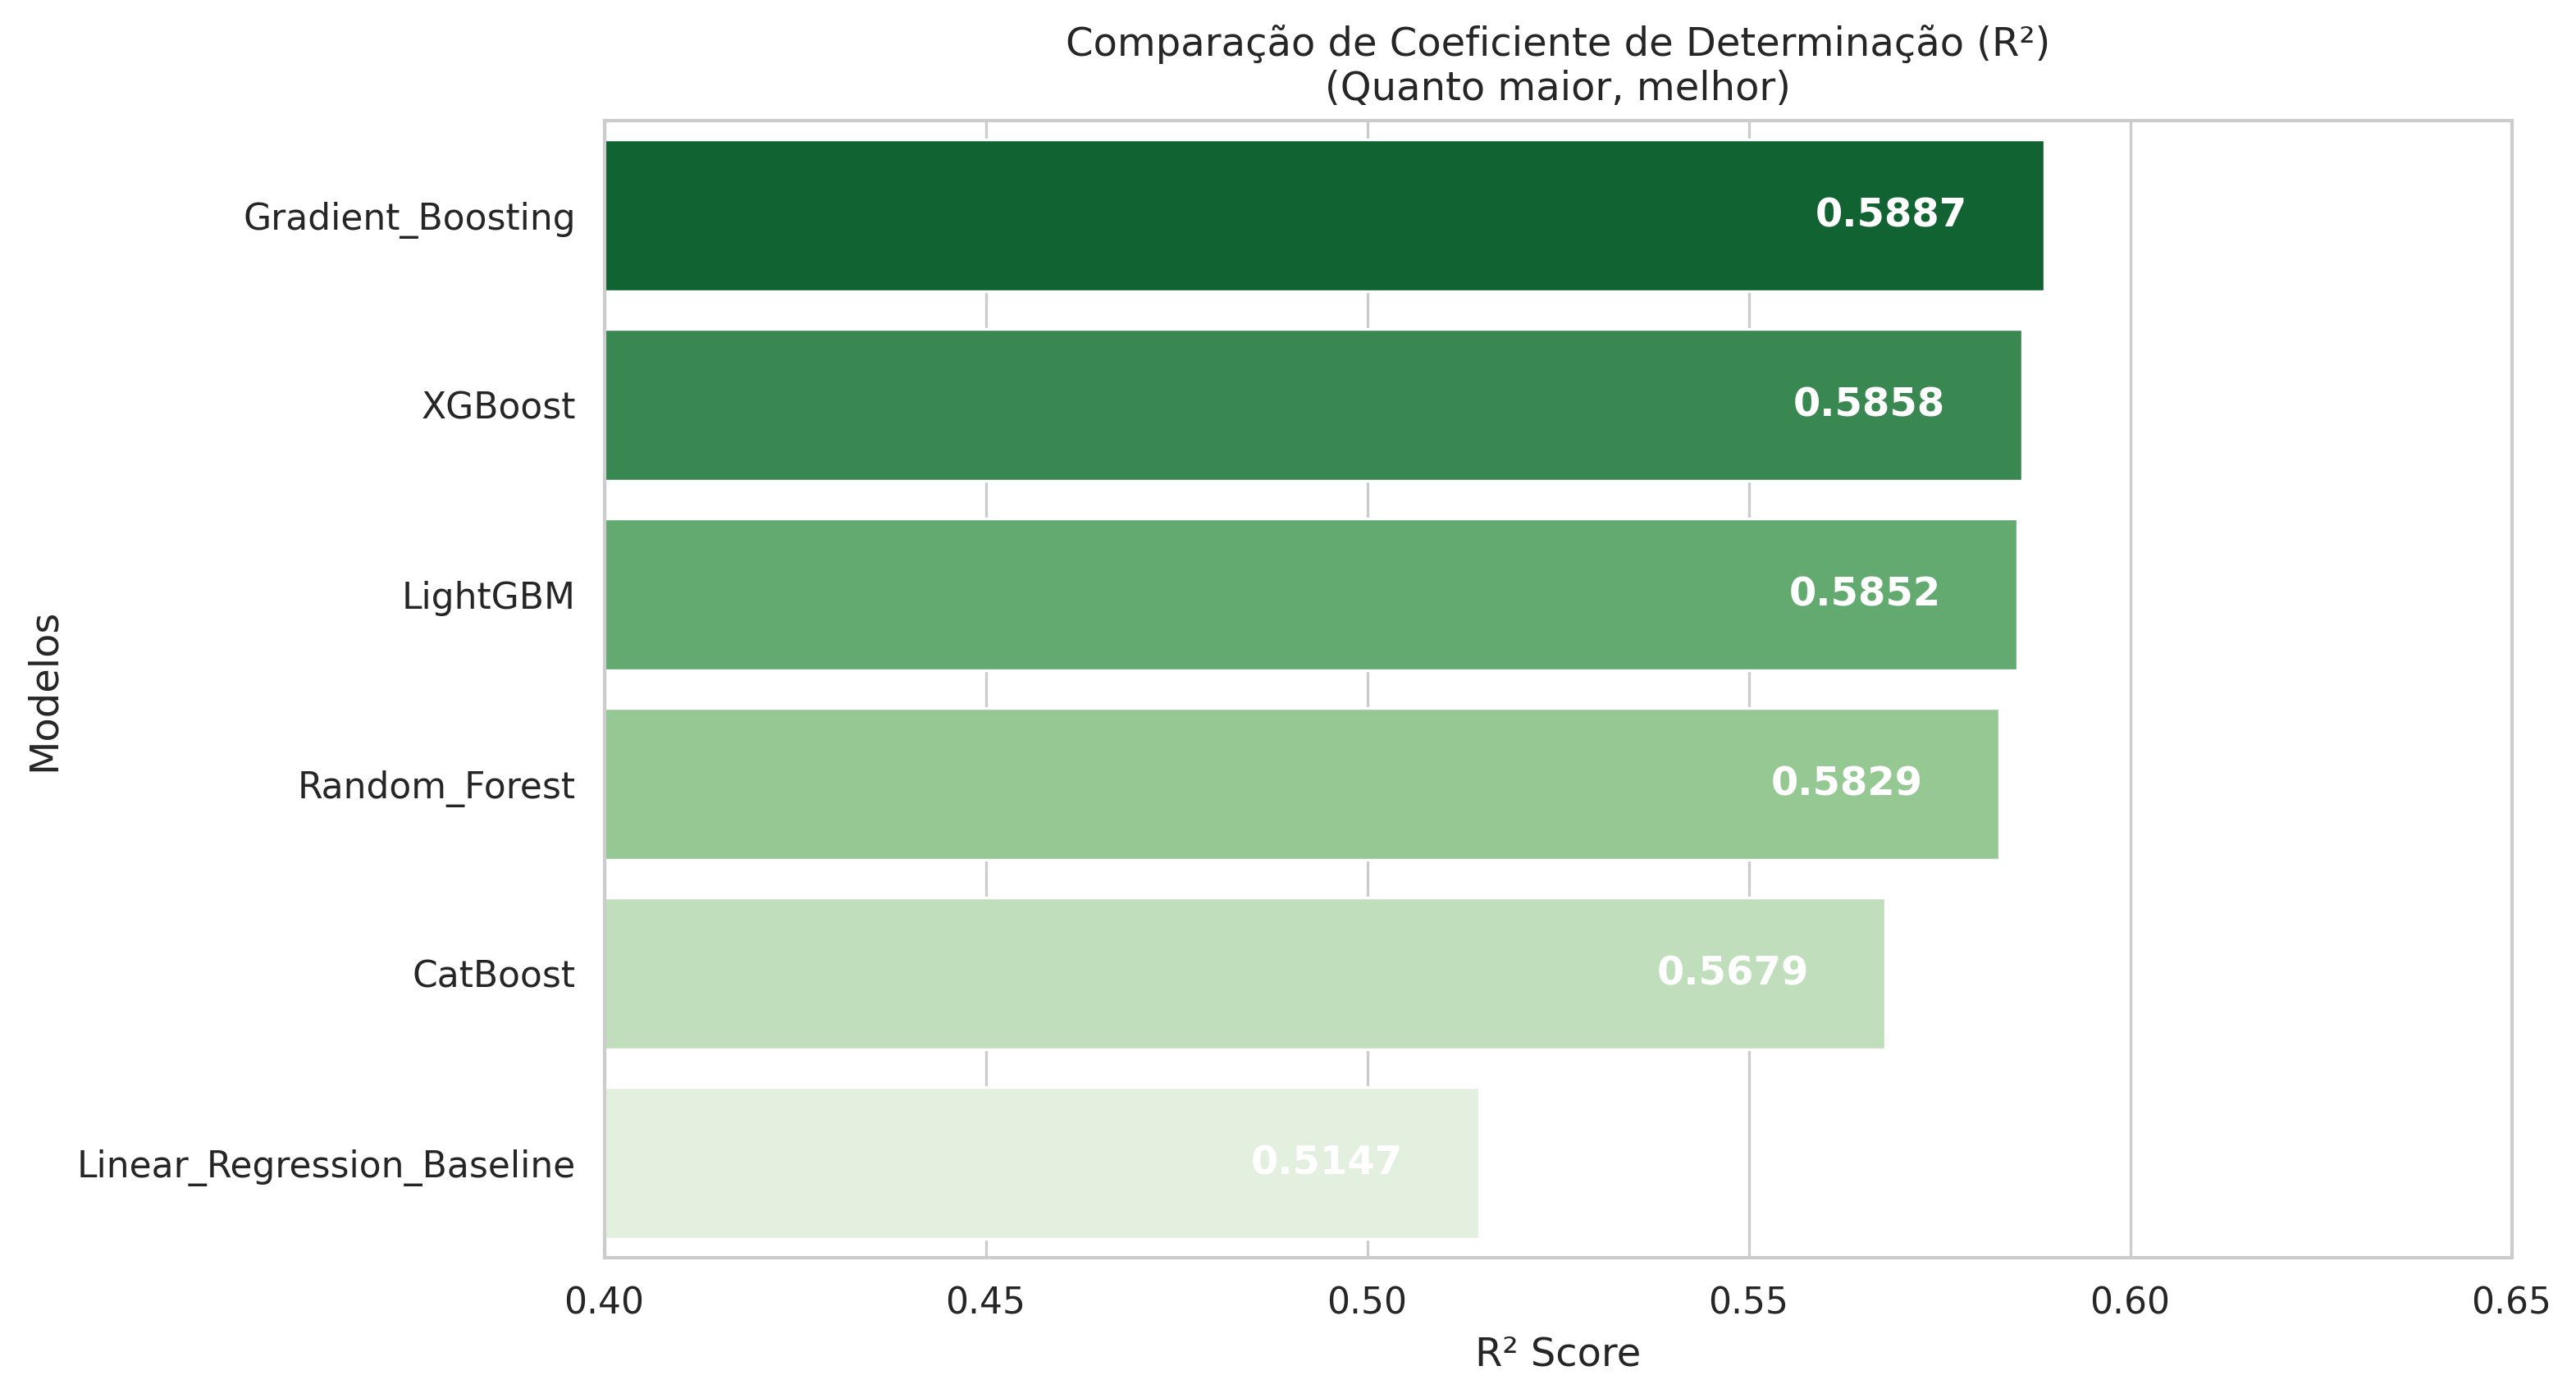
\includegraphics[width=1\linewidth]{images/comparativo_r2.png}
    \caption{Coefficient of Determination ($R^2$) comparison across the evaluated machine learning models.}
    \label{fig:comparativo_r2}
\end{figure}

As observed in Figures \ref{fig:comparativo_rmse} and \ref{fig:comparativo_r2}, all tree-based ensemble methods (Random Forest, Gradient Boosting, XGBoost, LightGBM, and CatBoost) significantly outperformed the Linear Regression baseline, which achieved an $R^2$ of 0.5147 and an RMSE of 38.23 kg. This substantial gap (an improvement of approximately 14\% in $R^2$ variance explained) underscores the highly non-linear nature of air traffic dynamics and the necessity of using advanced algorithms to capture complex interactions between arrival sectors, time of day, and congestion levels.

Among the ensemble methods, the performances were remarkably competitive. The standard Gradient Boosting Regressor (Scikit-Learn implementation) yielded the best overall results, reaching an $R^2$ of 0.5887 and an RMSE of 35.19 kg. It was closely followed by XGBoost and LightGBM. The slightly inferior performance of CatBoost in this specific setup ($R^2$ = 0.5679) can likely be attributed to the fact that we fed it a pre-encoded (One-Hot) dataset to maintain consistency across the benchmark, whereas CatBoost is specifically optimized to internally process native ordinal categorical data.

Overall, explaining nearly 59\% of the variance in additional fuel consumption ($KPI16$) indicates that a substantial portion of its variability can be explained by the selected operational, traffic, and meteorological variables. Predicting tactical fuel penalties prior to TMA entry enables controllers to anticipate bottlenecks and allows airlines to optimize their fuel policies dynamically.

\subsection{Hyperparameter Tuning and Optimization}
Following the baseline evaluation of the machine learning algorithms, an extensive hyperparameter tuning phase was conducted to maximize the predictive capability of the models. The default parameters, while robust, often fail to capture the nuances of complex non-linear relationships present in aviation datasets. This is especially true regarding the trade-off between the learning rate and the number of estimators, and the tendency of tree-based methods to overfit on dominant features such as the predicted transit time (\textit{transit\_tma\_predicted}).

To systematically explore the hyperparameter space, we employed Optuna \cite{akiba2019optuna}, an open-source hyperparameter optimization framework that utilizes Bayesian optimization. Unlike an exhaustive grid search, Optuna's Tree-structured Parzen Estimator (TPE) algorithm probabilistically samples the search space, focusing on regions that are more likely to yield optimal results, thus significantly reducing computational time while improving the search efficiency compared to exhaustive approaches.

\subsubsection{Optimization Strategy}
The tuning process was applied to all applicable tree-based ensemble methods: Random Forest, Gradient Boosting, XGBoost, LightGBM, and CatBoost. For each model, we defined an objective function to minimize the Mean Squared Error (MSE) using a 20\% validation hold-out set. The optimization trials ran iteratively, focusing on the following key aspects:

\begin{itemize}
    \item \textbf{Learning Rate and Estimators Trade-off:} We allowed the framework to explore lower learning rates paired with a higher number of estimators. This combination generally improves the model's ability to converge smoothly to a global minimum without overshooting.
    \item \textbf{Tree Complexity (Depth and Leaves):} The maximum depth of the trees (\textit{max\_depth}) and the maximum number of leaves (\textit{num\_leaves}) were expanded to allow the models to capture deeper, more intricate interactions among the spatial and temporal variables.
    \item \textbf{Regularization (L1/L2 Penalties):} To prevent the models from memorizing the training data, we introduced L1 (\textit{reg\_alpha}) and L2 (\textit{reg\_lambda} or \textit{l2\_leaf\_reg}) regularization terms. This forces the algorithms to keep the tree weights small and generalized.
    \item \textbf{Subsampling and Feature Selection:} We optimized the \textit{subsample} (fraction of rows used per tree) and \textit{colsample\_bytree} (fraction of columns used per tree) parameters. By restricting the models to around 60\% to 80\% of the data or features per iteration, we forced the ensembles to learn from diverse perspectives, reducing their over-reliance on the dominant \textit{transit\_tma\_predicted} feature.
\end{itemize}

\subsubsection{Tuning Results and Winning Model}
The optimization phase yielded substantial improvements across the gradient boosting algorithms, as detailed in Table \ref{tab:tuning_results}.

\begin{table}[htbp]
\caption{Model Performance ($R^2$) Before and After Hyperparameter Tuning}
\label{tab:tuning_results}
\centering
\begin{tabular}{lccc}
\hline
\textbf{Model} & \textbf{Baseline $R^2$} & \textbf{Tuned $R^2$} & \textbf{Improvement} \\
\hline
Linear Regression & 0.5147 & N/A & N/A \\
Random Forest & 0.5829 & 0.5852 & +0.23\% \\
Gradient Boosting & 0.5887 & 0.6212 & +3.25\% \\
LightGBM & 0.5852 & 0.6236 & +3.84\% \\
XGBoost & 0.5858 & 0.6248 & +3.90\% \\
\textbf{CatBoost} & \textbf{0.5679} & \textbf{0.6259} & \textbf{+5.80\%} \\
\hline
\end{tabular}
\end{table}

While the Random Forest algorithm saw only a marginal gain—a behavior that is common in bagging methods which are less sensitive to hyperparameter changes—all gradient boosting architectures experienced significant leaps in performance.

The most notable outcome of the tuning process was the performance of CatBoost. In the baseline evaluation, CatBoost placed last among the tree-based methods ($R^2$ = 0.5679), primarily because the dataset had been pre-processed with One-Hot Encoding to ensure a strict one-to-one benchmark against the other models, whereas CatBoost is natively optimized to handle raw categorical data internally. However, after undergoing Bayesian optimization with Optuna, CatBoost experienced a massive 5.80\% improvement in explained variance, jumping to the first position with an $R^2$ of 0.6259 and an RMSE of 33.56 kg.

These results solidify CatBoost as the winning model of this study. This dramatic leap in performance was heavily driven by the optimization of its specific hyperparameters. First, the number of \textit{iterations} was elevated to 900, coupled with a highly calibrated \textit{learning\_rate} of approximately 0.0596, allowing for steady convergence. The \textit{depth} of the oblivious trees was increased to 9, giving the model the ability to detect deeper conditional patterns without excessive branching. To prevent this increased depth from overfitting, the \textit{subsample} ratio was reduced to 0.734 (meaning each tree was trained on only ~73\% of the data) and the \textit{l2\_leaf\_reg} (L2 regularization coefficient) was refined. These optimized parameters allowed CatBoost to effectively navigate the complex categorical interactions (such as the relationship between specific departure airports and entry sectors) and deliver the most accurate estimations of additional fuel consumption in the Terminal Maneuvering Area.

\subsection{Feature Importance Analysis}
In predictive modeling for air traffic management, understanding the drivers behind a model's decisions is as critical as its overall accuracy. Figure \ref{fig:feature_importance} presents the aggregated feature importance extracted from the best-performing model, the tuned CatBoost regressor. Because the dataset was one-hot encoded, the importances of the dummy variables were aggregated by their base feature name to reflect the true weight of each categorical variable.

\begin{figure}[htbp]
    \centering
    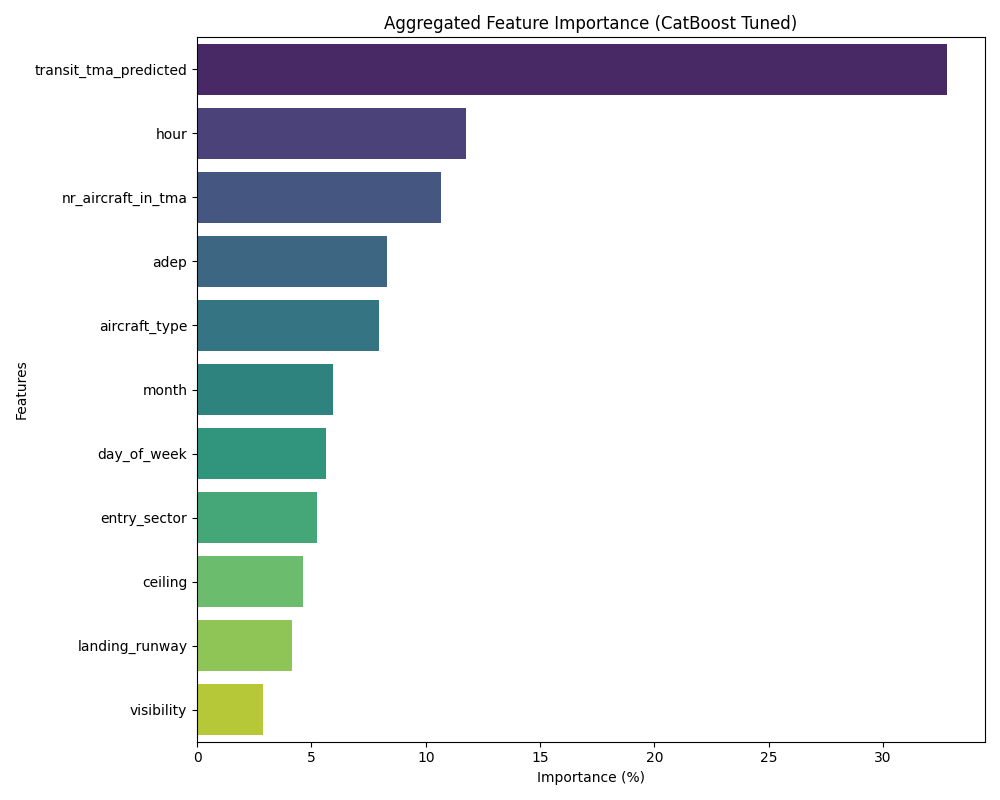
\includegraphics[width=1\linewidth]{images/feature_importance.png}
    \caption{Aggregated feature importance ranking from the tuned CatBoost model.}
    \label{fig:feature_importance}
\end{figure}

The analysis reveals that the moving average of predicted transit time in the TMA (\texttt{transit\_tma\_predicted}) is the most critical explanatory variable, accounting for nearly a third of the model's total predictive power. This outcome underscores the profound impact of airspace congestion on fuel consumption. By effectively tracking the historical density of approaching flights, this engineered feature captures operational conditions that may be associated with delays, holding patterns, or vectoring.

Following the transit time predictor, variables linked to air traffic schedules and volume—specifically the hour of the day (\texttt{hour}) and the concurrent number of aircraft in the TMA (\texttt{nr\_aircraft\_in\_tma})—demonstrate significant importance. These factors are likely associated with controller workload, traffic complexity and the likelihood of experiencing tactical delays upon arrival. Furthermore, the departure airport (\texttt{adep}) and aircraft type (\texttt{aircraft\_type}) hold considerable weight, as different origins imply distinct entry routes and sequencing challenges, while aircraft models inherently possess varied fuel flow capabilities and descent profiles.

Conversely, variables such as cloud ceiling (\texttt{ceiling}), validated landing runway (\texttt{landing\_runway}), and visibility (\texttt{visibility}) showed lower relative importance. While adverse meteorological conditions and runway configurations prompt Air Traffic Control to enforce greater separation minimums, the resulting delays are already largely captured by the primary traffic density metrics, mitigating their direct impact in the model.

\section{CONCLUSION}

In this paper, we successfully developed and validated a machine learning framework to estimate the additional fuel consumption (KPI16) during the terminal maneuvering area (TMA) operations at Guarulhos International Airport. By integrating real-world radar trajectories, BADA performance parameters, and existing operational metrics (such as KPI08) into a scalable data architecture, we created a robust and reproducible analytical pipeline.

The comparative analysis of gradient boosting algorithms demonstrated that the LightGBM model achieved the most effective balance of predictive performance and generalization, with an $R^2$ of 0.64 and a mean absolute error of 17.85 kg. Furthermore, our feature importance analysis highlighted that the predicted transit time within the TMA was the most significant explanatory variable. This finding underscores the direct impact of air traffic congestion and sequencing inefficiencies on both environmental and operational costs.

The resulting methodology provides a reliable tool for the continuous monitoring of operational efficiency, aligning with international sustainability goals and the performance-based management advocated by ICAO. Future work will focus on expanding the scope of the model to encompass other aircraft families and major airports. Additionally, we plan to incorporate real-time meteorological conditions and air traffic flow management (ATFM) data to further enhance predictive accuracy, and to deploy the model within institutional dashboards for automated, near real-time KPI monitoring.

\bibliographystyle{IEEEtran}
\bibliography{chapters/references}

\end{document}